% Created with jtex v.1.0.21
\documentclass{article}
\usepackage{hyperref}
\usepackage{datetime}
\usepackage{graphicx}
\usepackage{natbib}
\bibliographystyle{abbrvnat}

%%%%%%%%%%%%%%%%%%%%%%%%%%%%%%%%%%%%%%%%%%%%%%%%%%
%%%%%%%%%%%%%%%%%%%%  imports  %%%%%%%%%%%%%%%%%%%
\usepackage{amsmath}
\usepackage{booktabs}
\usepackage{framed}
\usepackage{url}
%%%%%%%%%%%%%%%%%%%%%%%%%%%%%%%%%%%%%%%%%%%%%%%%%%


% colors for hyperlinks
\hypersetup{colorlinks=true, allcolors=blue}

\newcommand{\logo}{
  \href{https://curvenote.com}{
\includegraphics[width=2cm]{curvenote.png}}
}

\title{Projeto Hermathena}

\author{Luciano Barosi}

\newdate{articleDate}{10}{3}{2026}
\date{\displaydate{articleDate}}

\begin{document}
\maketitle
\begin{center}\logo\end{center}


\section{Ecossistema Hermathena}

O Projeto Hermathena organiza as ações de comunicação científica do radiotelescópio \textbf{BINGO} como um ecossistema integrado de núcleos especializados.

Cada núcleo atua em uma dimensão específica da comunicação científica, permitindo transformar a presença do radiotelescópio no sertão paraibano em uma plataforma de \textbf{educação, inovação e desenvolvimento regional}.

\section{Ecossistema do Projeto Hermathena}

O Projeto Hermathena está estruturado como um ecossistema integrado de comunicação científica, educação e tecnologia.

\begin{verbatim}
O Projeto Hermathena está estruturado como um ecossistema integrado de comunicação científica, educação e tecnologia.

```mermaid
flowchart TB

    BINGO[🔭 Radiotelescópio BINGO]

    BINGO - -> VIA[🌌 Via Láctea<br>Comunicação Educacional]
    BINGO - -> AND[🌠 Andromeda<br>Engajamento Digital]
    BINGO - -> TRI[🔭 Triangulum<br>Conteúdo Profundo]
    BINGO - -> MAG[🛰 Magellan<br>Infraestrutura Digital]

    VIA - -> EDU[Materiais educacionais]
    AND - -> SOCIAL[Redes sociais]
    TRI - -> VIDEO[Podcasts e documentários]
    MAG - -> PORTAL[Portal e sistemas]

flowchart TB

    BINGO[🔭 Radiotelescópio BINGO]

    BINGO - -> VIA[🌌 Via Láctea<br>Comunicação Educacional]
    BINGO - -> AND[🌠 Andromeda<br>Engajamento Digital]
    BINGO - -> TRI[🔭 Triangulum<br>Conteúdo Profundo]
    BINGO - -> MAG[🛰 Magellan<br>Infraestrutura Digital]

    VIA - -> EDU[Materiais educacionais]
    AND - -> SOCIAL[Redes sociais]
    TRI - -> VIDEO[Podcasts e documentários]
    MAG - -> PORTAL[Portal e sistemas]
\end{verbatim}

\section{Geral}

\subsection{Motivação}

O projeto \textbf{Hermathena} nasce da confluência entre dois domínios que, à primeira vista, parecem distantes: a ciência de fronteira e a comunicação popular. Seu nome evoca precisamente essa fusão. \textit{Hermathena} é um termo cunhado por Cícero, no século I a.C., para descrever uma escultura que combinava as figuras de \textbf{Hermes} --- deus da comunicação, das mensagens e das travessias --- e \textbf{Atena} --- deusa da sabedoria, da ciência e das artes. Para Cícero, a peça representava o ideal de que o conhecimento e a eloquência são inseparáveis: não basta saber, é preciso saber comunicar.

É com esse espírito que o projeto Hermathena se propõe a construir pontes entre a pesquisa científica de excelência conduzida no âmbito do Radiotelescópio BINGO e a sociedade paraibana --- em especial as comunidades do sertão que convivem, literalmente, com um dos instrumentos científicos mais sofisticados já construídos no Brasil.

O projeto é um desdobramento direto do Programa de Extensão BINGO (PROBEX/UFCG), e emerge num momento em que o investimento em ciência e tecnologia no Estado da Paraíba alcança uma escala histórica, articulando instituições de ensino, esferas de governo e parceiros internacionais em torno de três grandes iniciativas:

\begin{itemize}
\item O \textbf{Radiotelescópio BINGO}, em Aguiar;
\item A \textbf{Cidade da Astronomia}, em Carrapateira;
\item O \textbf{Centro de Computação Quântica}, em fase de planejamento.
\end{itemize}

Diante desse cenário, comunicar ciência deixa de ser uma obrigação burocrática e torna-se um ato político e pedagógico: é a condição para que o desenvolvimento científico se converta em desenvolvimento humano.


\bigskip
\centerline{\rule{13cm}{0.4pt}}
\bigskip

\subsubsection{1.2 Missão}

Estabelecer as bases para garantir, registrar e potencializar as ações das equipes envolvidas com o Radiotelescópio BINGO, conducentes à materialização do projeto como vetor de desenvolvimento humano, científico, educacional e econômico no Estado da Paraíba e região Nordeste.

Este significado foi rapidamente compreendido pelos membros da colaboração, pelos gestores das instituições públicas de ensino da Paraíba, por órgãos de fomento e, sobretudo, pelo Governo do Estado da Paraíba, que aportou recursos significativos além de planejar e iniciar obras estruturantes no alto sertão --- com a pavimentação das rodovias do entorno do radiotelescópio e com a criação do projeto Cidade da Astronomia, no município de Carrapateira.

O Radiotelescópio BINGO é, por natureza, um projeto inter e transdisciplinar. Sua construção e operação mobilizam simultaneamente competências em física, engenharia, computação, ciências ambientais, ciências sociais e comunicação --- áreas que não apenas coexistem, mas precisam dialogar para que o projeto cumpra seu potencial. Essa característica se reflete diretamente na estrutura do projeto Hermathena, que reúne equipes de diferentes instituições --- UFCG, UFPB, UEPB, IFPB, além de parceiros internacionais --- numa prática genuína de ciência colaborativa, em que o conhecimento é produzido e compartilhado de forma distribuída, superando fronteiras disciplinares e institucionais.

Mais do que um feito científico, a instalação do BINGO no sertão paraibano representa uma oportunidade concreta de enfrentamento de demandas históricas da população regional: a escassez de oportunidades educacionais e profissionais em uma das regiões mais carentes do estado, a ausência de infraestrutura tecnológica e a distância entre as comunidades locais e os circuitos de produção do conhecimento. Nesse sentido, o esforço de comunicação científica proposto pelo Hermathena é também um esforço educacional --- voltado para despertar vocações científicas e tecnológicas nas novas gerações, fortalecer a formação de professores da educação básica e criar laços duradouros entre a universidade e a sociedade do sertão.

É fundamental, portanto, que esse movimento de investimento público e científico seja acompanhado por uma comunicação à altura: capaz de explicar à sociedade o que está sendo construído em seu território, de engajar as comunidades locais como protagonistas desse processo e de traduzir a linguagem da ciência de fronteira em oportunidades concretas de desenvolvimento humano e regional.

\subsubsection{1.3 Pilares Estratégicos}

\bigskip\noindent
\begin{tabular}{p{\dimexpr 0.333\linewidth-2\tabcolsep}p{\dimexpr 0.333\linewidth-2\tabcolsep}p{\dimexpr 0.333\linewidth-2\tabcolsep}}
\toprule
Pilar & Descrição & Público-Alvo \\
\hline
\textbf{Educação} & Formação em STEM e cosmologia para educação básica & Estudantes e educadores \\
\textbf{Pesquisa} & Divulgação de resultados científicos e metodologias & Comunidade acadêmica \\
\textbf{Extensão} & Integração com comunidades locais e regionais & Sociedade paraibana \\
\textbf{Inovação} & Transferência tecnológica e atração de investimentos & Setor produtivo \\
\bottomrule
\end{tabular}

\bigskip

\subsubsection{1.4 Objetivos de Desenvolvimento Sustentável (ODS)}

O projeto contempla diretamente os seguintes ODS da Agenda 2030:

\begin{itemize}
\item \textbf{ODS 4:} Educação de Qualidade
\item \textbf{ODS 9:} Indústria, Inovação e Infraestrutura
\item \textbf{ODS 10:} Redução das Desigualdades
\item \textbf{ODS 17:} Parcerias e Meios de Implementação
\end{itemize}


\bigskip
\centerline{\rule{13cm}{0.4pt}}
\bigskip

\subsection{Contexto: O Radiotelescópio BINGO}

\subsubsection{O que é o BINGO?}

O \textbf{BINGO} (Baryon Acoustic Oscillations in Neutral Gas Observations) é um radiotelescópio de última geração projetado para realizar a primeira detecção de Oscilações Acústicas de Bárions (BAO) na faixa de radiofrequência.

\paragraph{Características Técnicas}

\bigskip\noindent
\begin{tabular}{p{\dimexpr 0.500\linewidth-2\tabcolsep}p{\dimexpr 0.500\linewidth-2\tabcolsep}}
\toprule
Característica & Especificação \\
\hline
\textbf{Tipo} & Radiotelescópio de mapeamento de intensidade \\
\textbf{Frequência} & 980 - 1260 MHz \\
\textbf{Espelho primário} & 40 metros de diâmetro \\
\textbf{Espelho secundário} & 35 metros de diâmetro \\
\textbf{Receptores} & 28 cornetas no plano focal \\
\textbf{Campo de visada} & 15° em declinação \\
\textbf{Operação} & Drift-scan (sem partes móveis) \\
\bottomrule
\end{tabular}

\bigskip

\paragraph{Localização}

O telescópio está sendo instalado na \textbf{Serra do Urubu}, município de \textbf{Aguiar}, no Vale do Piancó, Sertão da Paraíba. A escolha do local considerou:

\begin{itemize}
\item Baixa poluição eletromagnética
\item Ausência de sinal de celular nas proximidades
\item Sem rotas aéreas diretas
\item Colaboração da comunidade local
\item Acesso viável para manutenção
\end{itemize}

\paragraph{Missão Científica}

O BINGO foi concebido para responder algumas das perguntas mais fundamentais da cosmologia contemporânea.

O BINGO investigará:

\begin{enumerate}
\item \textbf{Energia Escura}: Componente misteriosa que acelera a expansão do universo
\item \textbf{Matéria Escura}: Matéria invisível que influencia a estrutura cósmica
\item \textbf{Oscilações Acústicas de Bárions (BAO)}: ``Marcadores padrão'' do universo
\item \textbf{Rajadas Rápidas de Rádio (FRB)}: Eventos energéticos misteriosos
\end{enumerate}

\subsubsection{Colaboração Internacional}

O projeto é uma parceria entre:

\bigskip\noindent
\begin{tabular}{p{\dimexpr 0.333\linewidth-2\tabcolsep}p{\dimexpr 0.333\linewidth-2\tabcolsep}p{\dimexpr 0.333\linewidth-2\tabcolsep}}
\toprule
País & Instituições Principais & Contribuição \\
\hline
\textbf{Brasil} & USP, INPE, UFCG, UFPB & Coordenação científica, instalação, operação \\
\textbf{Reino Unido} & Universities of Manchester, Oxford & Instrumentação, análise de dados \\
\textbf{China} & CAS, Yangzhou University & Espelhos, estrutura mecânica \\
\textbf{Suíça} & FHNW & Eletrônica de receptor \\
\textbf{África do Sul} & SARAO & Troca de expertise em radioastronomia \\
\bottomrule
\end{tabular}

\bigskip

\subsubsection{Significado para o Brasil}

O BINGO representa:

\begin{itemize}
\item \textbf{Primeiro radiotelescópio} dessa magnitude construído no Brasil
\item \textbf{Inovação industrial} com fabricação nacional de componentes
\item \textbf{Formação de recursos humanos} em radioastronomia
\item \textbf{Desenvolvimento regional} no Sertão paraibano
\item \textbf{Inserção internacional} da ciência brasileira em cosmologia
\end{itemize}

\subsubsection{Linha do Tempo}

\bigskip\noindent
\begin{tabular}{p{\dimexpr 0.500\linewidth-2\tabcolsep}p{\dimexpr 0.500\linewidth-2\tabcolsep}}
\toprule
Ano & Marco \\
\hline
2017 & Aprovação da colaboração BINGO \\
2019 & Início das obras no sítio em Aguiar \\
2022 & Inauguração formal do projeto \\
2024 & Chegada dos componentes da China \\
2025-2026 & Montagem e testes do telescópio \\
2027 & Primeiras observações científicas \\
\bottomrule
\end{tabular}

\bigskip

\subsubsection{Recursos}

\begin{itemize}
\item \textbf{Site oficial:} \href{https://bingotelescope.org}{https://bingotelescope.org}
\item \textbf{Coordenação Brasil:} Prof. Elcio Abdalla (USP)
\item \textbf{Coordenação UFCG:} Prof. Edmar Candeia Gurjão (DEE/UFCG)
\item \textbf{Coordenação Hermathena:} Luciano Barosi
\end{itemize}

\subsubsection{É neste contexto que surge o projeto Hermathena, concebido para transformar a presença do radiotelescópio BINGO no sertão paraibano em uma oportunidade ampliada de educação científica, comunicação pública da ciência e desenvolvimento regional.}

\textit{Para mais informações técnicas, consulte a documentação científica da colaboração BINGO.}

\section{Organizacao}

\subsection{Estrutura Organizacional}

\subsubsection{2. Estrutura Organizacional}

Hermathena = Ecossistema de Comunicação Científica

Laniakea  \rightarrow Governança
Virgo     \rightarrow Steering Committee

Magellan  \rightarrow Tecnologia
Via Láctea \rightarrow Educação
Andromeda \rightarrow Engajamento
Triangulum \rightarrow Conteúdo profundo

\begin{figure}[!htbp]
\centering
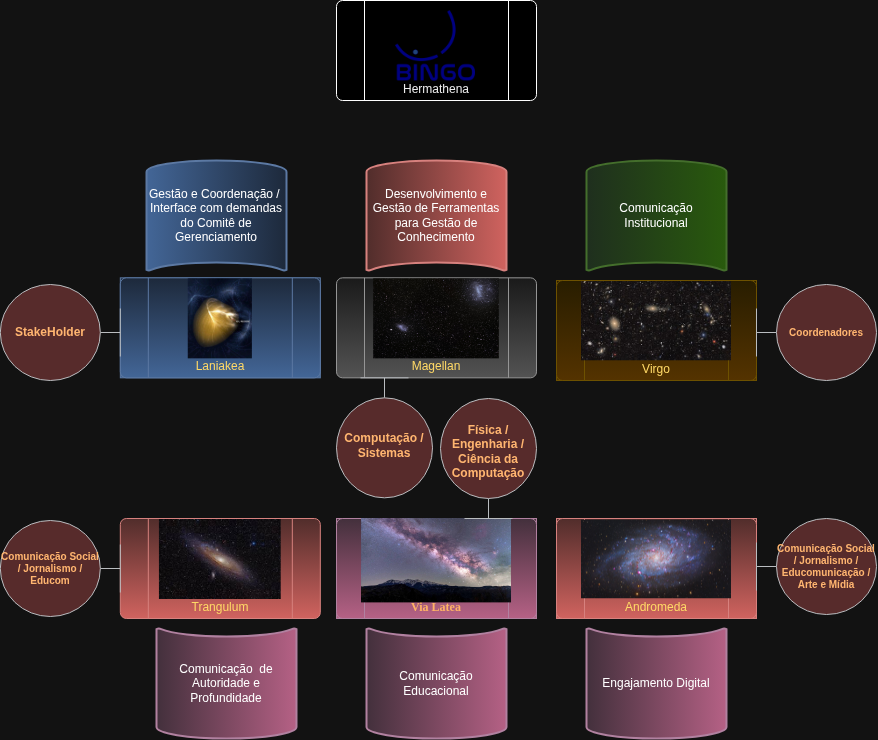
\includegraphics[width=1\linewidth]{files/nucleos-b9222e3152f6e2ffed5593f446132d20.png}
\end{figure}

\paragraph{2.1 Núcleos de Atuação}

O projeto está organizado em \textbf{núcleos}, cada um com funções específicas, complementares e afinidade de área definida.

\subparagraph{Núcleo 0: Laniakea}

Corresponde aos stakeholders do projeto. É constituído por representantes dos coordenadores do projeto juntamente com representantes do gerenciamento do projeto radiotelescópio BINGO e demais atores relevantes, a exemplo de financiadores.

\subparagraph{Núcleo 1: Magellan --- Ferramentas TIC}

Encarregado de promover um workflow para os demais projetos que garanta a qualidade das informações, sua temporalidade, reservas de direito, promoção de uma boa experiência para os usuários de todos os níveis.

\bigskip\noindent
\begin{tabular}{p{\dimexpr 0.500\linewidth-2\tabcolsep}p{\dimexpr 0.500\linewidth-2\tabcolsep}}
\toprule
Atributo & Descrição \\
\hline
\textbf{Afinidade de Área} & Ciência da Computação / Análise e Desenvolvimento de Sistemas \\
\textbf{Função} & Desenvolvimento de ferramentas tecnológicas \\
\textbf{Responsabilidades} & Criação e manutenção de sistemas; Automação de tarefas; Desenvolvimento de soluções; UI/UX \\
\textbf{Produtos} & Portal web, sistemas de automação, dashboards, chatbot, app mobile \\
\bottomrule
\end{tabular}

\bigskip

\subparagraph{Núcleo 2: Virgo --- Steering Committee}

Este é o local de troca de informações dos coordenadores de todos os projetos, pode começar com uma estrutura muito enxuta, mas assume cada vez mais relevância ao agregarmos parceiros de outras instituições

\bigskip\noindent
\begin{tabular}{p{\dimexpr 0.500\linewidth-2\tabcolsep}p{\dimexpr 0.500\linewidth-2\tabcolsep}}
\toprule
Atributo & Descrição \\
\hline
\textbf{Composição} & Membro designado do grupo de gerenciamento do BINGO (ouvinte); profissionais de comunicação convidados; 1 membro do projeto de cada instituição parceira \\
\textbf{Função} & Coordenação estratégica e governança \\
\textbf{Responsabilidades} & Definição de diretrizes estratégicas; Aprovação de grandes decisões; Interface com colaboração BINGO internacional; Supervisão de resultados \\
\bottomrule
\end{tabular}

\bigskip

\subparagraph{Núcleo 3: Via Láctea --- Comunicação Educacional}

\bigskip\noindent
\begin{tabular}{p{\dimexpr 0.500\linewidth-2\tabcolsep}p{\dimexpr 0.500\linewidth-2\tabcolsep}}
\toprule
Atributo & Descrição \\
\hline
\textbf{Afinidade de Área} & Física / Engenharia Elétrica \\
\textbf{Função} & Comunicação educacional \\
\textbf{Responsabilidades} & Produção de material educacional; Construção de equipamentos de demonstração; conteúdo para Portal web; elaboração de roteiros, manuais, planos de experiências... \\
\textbf{Produtos} & Portal web, biblioteca educacional, manuais, equipamentos de demonstração \\
\bottomrule
\end{tabular}

\bigskip

\subparagraph{Núcleo 4: Andromeda --- Comunicação de Engajamento}

\bigskip\noindent
\begin{tabular}{p{\dimexpr 0.500\linewidth-2\tabcolsep}p{\dimexpr 0.500\linewidth-2\tabcolsep}}
\toprule
Atributo & Descrição \\
\hline
\textbf{Afinidade de Área} & Comunicação Social / Educomunicação / Arte e Mídia / Jornalismo \\
\textbf{Função} & Comunicação de engajamento digital \\
\textbf{Responsabilidades} & Gestão de redes sociais (Instagram, Facebook, TikTok); Produção de conteúdo viral; Interação com comunidade online; Métricas de engajamento \\
\textbf{Produtos} & Feed Instagram, Facebook, Reels, TikToks, campanhas temáticas \\
\bottomrule
\end{tabular}

\bigskip

\subparagraph{Núcleo 5: Triangulum --- Comunicação de Profundidade}

\bigskip\noindent
\begin{tabular}{p{\dimexpr 0.500\linewidth-2\tabcolsep}p{\dimexpr 0.500\linewidth-2\tabcolsep}}
\toprule
Atributo & Descrição \\
\hline
\textbf{Afinidade de Área} & Comunicação Social / Educomunicação / Arte e Mídia / Jornalismo / Cinema \\
\textbf{Função} & Comunicação de profundidade e autoridade \\
\textbf{Responsabilidades} & Produção audiovisual longo; Canais de streaming; Entrevistas e debates; Documentários e séries \\
\textbf{Produtos} & Podcasts Spotify, vídeos YouTube, documentários, webinários, lives \\
\bottomrule
\end{tabular}

\bigskip

Do ponto de vista da aplicação do programa ao PROBEX/UFCG, o núcleo \textit{Virgo} representa a coordenação do programa e os núcleos \textit{Magellan}, \textit{Triangullum}, \textit{Via Lactea} e \textit{Andromeda} representam os projetos.

\paragraph{2.2 Estrutura das Equipes}

Cada núcleo operacional (Via Láctea, Andromeda, Triangulum, Magellan) possui:

\bigskip\noindent
\begin{tabular}{p{\dimexpr 0.333\linewidth-2\tabcolsep}p{\dimexpr 0.333\linewidth-2\tabcolsep}p{\dimexpr 0.333\linewidth-2\tabcolsep}}
\toprule
Função & Quantidade & Perfil \\
\hline
\textbf{Professor Orientador} & 1 & Docente da área de afinidade \\
\textbf{Professor Colaborador} & 1 & Docente de área complementar \\
\textbf{Bolsista PROBEX} & 1 & Graduação na área de afinidade \\
\textbf{Voluntários} & 5 & Graduação em áreas afins \\
\bottomrule
\end{tabular}

\bigskip

\textbf{Expansão:} Os núcleos podem se replicar em instituições parceiras, atingindo até \textbf{12 alunos + 4 docentes} por núcleo distribuídos.

\paragraph{2.3 Dinâmica de Trabalho}

\bigskip\noindent
\begin{tabular}{p{\dimexpr 0.250\linewidth-2\tabcolsep}p{\dimexpr 0.250\linewidth-2\tabcolsep}p{\dimexpr 0.250\linewidth-2\tabcolsep}p{\dimexpr 0.250\linewidth-2\tabcolsep}}
\toprule
Reunião & Frequência & Participantes & Modalidade \\
\hline
\textbf{Núcleo - Reunião de Produção} & Quinzenal & Membros do núcleo & Presencial \\
\textbf{Núcleo - Reunião de Acompanhamento} & Quinzenal & Membros do núcleo & Online \\
\textbf{Steering Committee (Virgo)} & Mensal & Coordenadores de núcleos & Online \\
\textbf{Laniakea} & Trimestral & Membros do comitê & Online \\
\bottomrule
\end{tabular}

\bigskip

\subsection{Eixos Temáticos de Conteúdo}

\begin{figure}[!htbp]
\centering
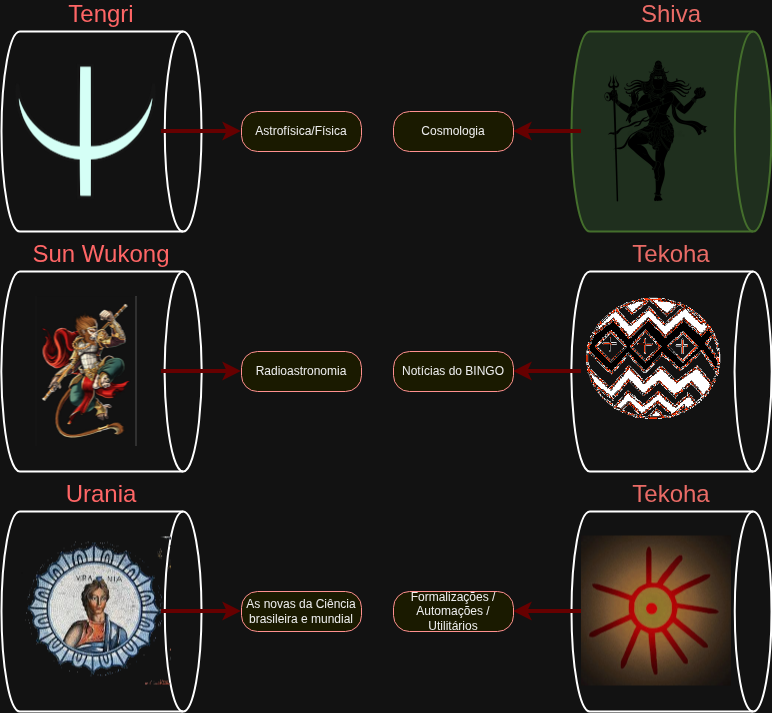
\includegraphics[width=1\linewidth]{files/eixos-dab8b38ab807d2296e5902c857fb6f08.png}
\end{figure}

\subsubsection{Conteúdos por Eixo}

\begin{itemize}
\item \textbf{Tengre:}

\begin{itemize}
\item Como medimos distâncias em astronomia,
\item Evolução de estrelas,
\item Pulsares,
\item Fenômenos transientes de Rádio,
\item Pulsar Timing Array,
\item Ondas Gravitacionais
\end{itemize}


\item \textbf{Shiva Nataraja:}

\begin{itemize}
\item A história térmica do universo,
\item Desacoplamento e recombinação,
\item Composição do Universo,
\item Matéria escura,
\item Energia escura,
\item Tensão de Hubble
\end{itemize}


\item \textbf{Sun Wukong:}

\begin{itemize}
\item Espectro eletromagnético,
\item Antenas e receptores,
\item Sinais digitais de rádio,
\item Interferências eletromagnéticas,
\item Planejamento de observações,
\item Espectrômetro,
\item Hidrogênio neutro
\end{itemize}


\item \textbf{Tekoha:}

\begin{itemize}
\item Editais e calendário,
\item Publicações,
\item Premiações,
\item Agenda de Eventos,
\item Modelos digitais,
\item Andamento da construção,
\item Notícias das Universidades,
\item Bolsistas
\end{itemize}


\item \textbf{Urania:}

\begin{itemize}
\item Notícias internacionais,
\item Clipping de ciência,
\item Featured article of the month
\end{itemize}


\item \textbf{Guaraci:}

\begin{itemize}
\item Portal,
\item Templates,
\item Workflows,
\item Automação,
\item Relatórios,
\item Press releases,
\item Apresentações para financiadores
\end{itemize}
\end{itemize}


\bigskip
\centerline{\rule{13cm}{0.4pt}}
\bigskip

\subsection{Núcleo Magellan: Ferramentas TIC}

\begin{figure}[!htbp]
\centering
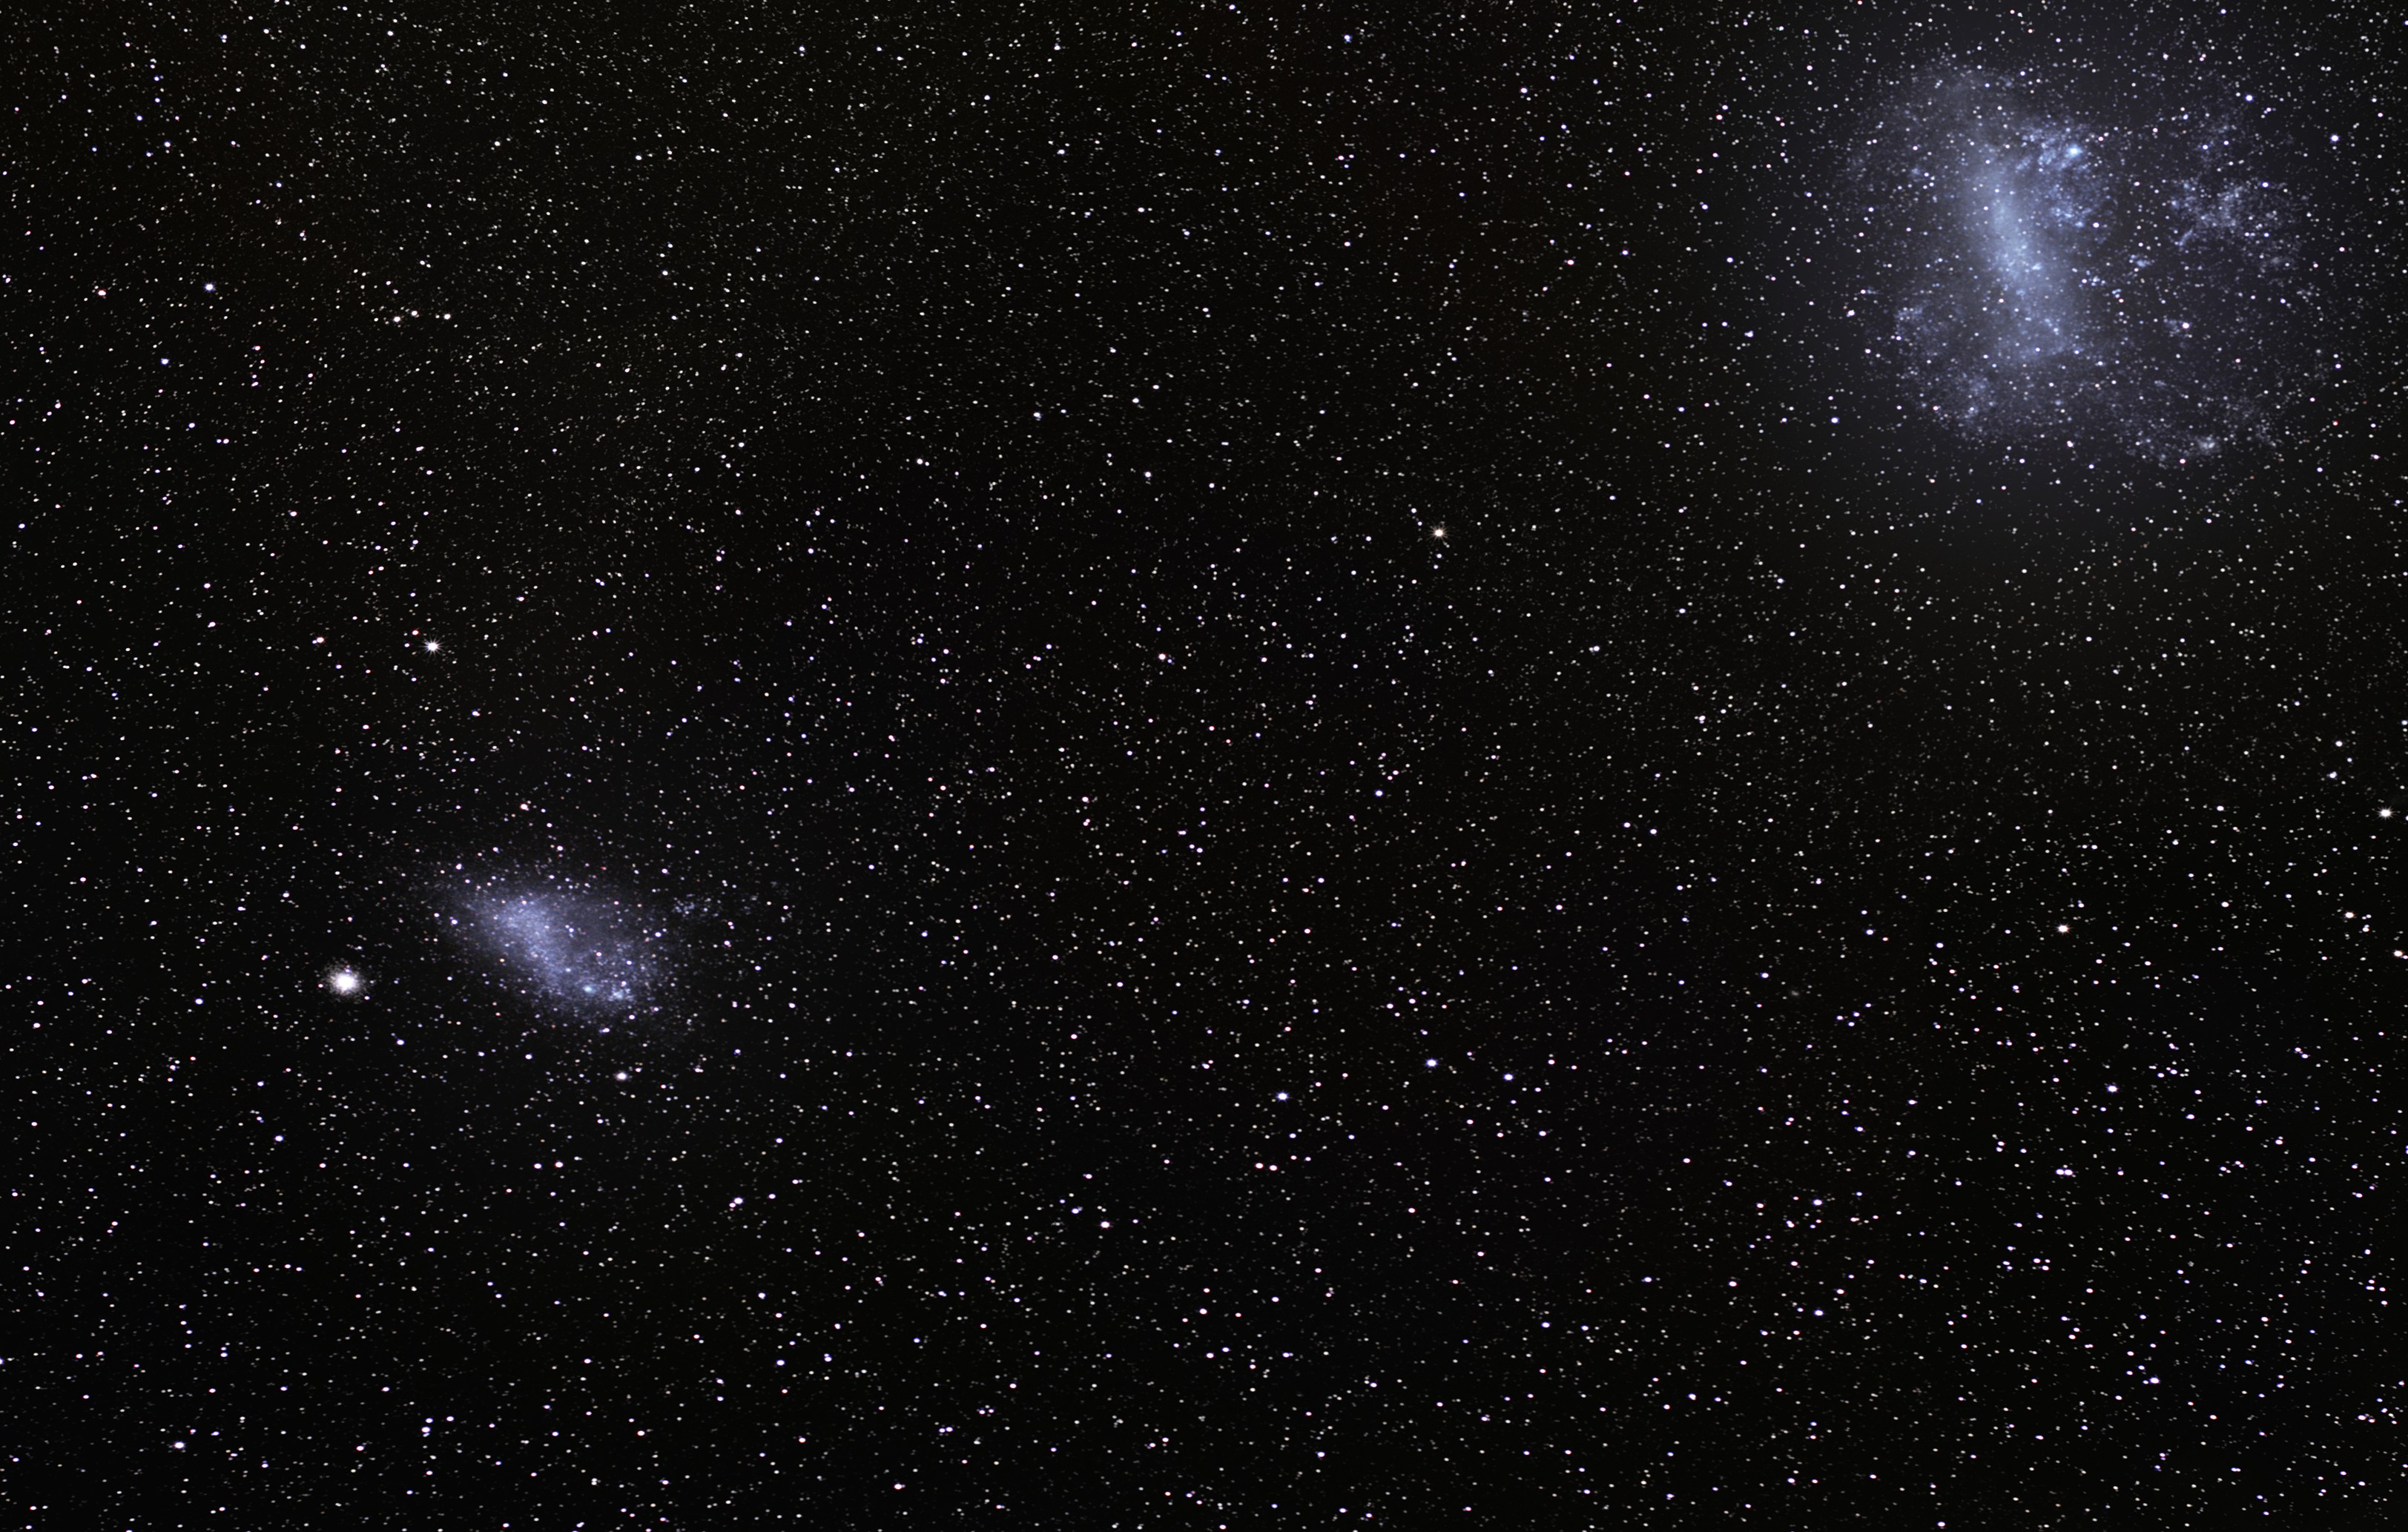
\includegraphics[width=1\linewidth]{files/magellan-d12d937615ed23573ffa3452b507cd3b.jpg}
\end{figure}

\subsubsection{Visão Geral}

O \textbf{Núcleo Magellan} é responsável pelo desenvolvimento e manutenção das ferramentas tecnológicas de informação e comunicação do Projeto Hermathena. Seu nome evoca as nuvens de Magalhães, símbolo de navegação e orientação, representando nossa missão de criar soluções digitais que guiem e potencializem todo o projeto.

\textbf{Afinidade de Área:} Ciência da Computação / Análise e Desenvolvimento de Sistemas / Engenharia de Software

\subsubsection{Missão}

Desenvolver, implementar e manter soluções tecnológicas que automatizem processos, facilitem a gestão de conteúdos e proporcionem experiências digitais inovadoras para os diferentes públicos do BINGO.

\subsubsection{Objetivos Específicos}

\paragraph{1. Desenvolvimento de Sistemas}

\subparagraph{1.1 Portal Web BINGO}

\begin{itemize}
\item[$\square$] Desenvolvimento do site institucional integrado
\item[$\square$] Sistema de gestão de conteúdo (CMS) customizado
\item[$\square$] Área administrativa para equipe
\item[$\square$] Integração com redes sociais
\item[$\square$] Otimização para SEO e acessibilidade
\end{itemize}

\subparagraph{1.2 Sistemas de Automação}

\begin{itemize}
\item[$\square$] Automação de publicações em redes sociais
\item[$\square$] Sistema de agendamento e calendário editorial
\item[$\square$] Automação de relatórios e métricas
\item[$\square$] Chatbot para atendimento e FAQ
\item[$\square$] Integração com APIs de plataformas
\end{itemize}

\subparagraph{1.3 Ferramentas Internas}

\begin{itemize}
\item[$\square$] Sistema de gestão de documentos
\item[$\square$] Dashboard de acompanhamento de indicadores
\item[$\square$] Ferramenta de versionamento colaborativo
\item[$\square$] Sistema de tickets e demandas
\item[$\square$] Wiki interna do projeto
\end{itemize}

\paragraph{2. Infraestrutura Digital}

\subparagraph{2.1 Servidores e Hospedagem}

\bigskip\noindent
\begin{tabular}{p{\dimexpr 0.333\linewidth-2\tabcolsep}p{\dimexpr 0.333\linewidth-2\tabcolsep}p{\dimexpr 0.333\linewidth-2\tabcolsep}}
\toprule
Componente & Especificação & Custo Estimado \\
\hline
\textbf{Servidor NAS} & Synology DS1821+ ou similar, 5x HDD 4TB & R\$ 20.000,00 \\
\textbf{Hospedagem Cloud} & VPS 4vCPU, 8GB RAM, 200GB SSD & R\$ 300,00/mês \\
\textbf{Backup em Nuvem} & 50TB storage + backup automático & R\$ 500,00/mês \\
\bottomrule
\end{tabular}

\bigskip

\subparagraph{2.2 Serviços de IA}

\bigskip\noindent
\begin{tabular}{p{\dimexpr 0.333\linewidth-2\tabcolsep}p{\dimexpr 0.333\linewidth-2\tabcolsep}p{\dimexpr 0.333\linewidth-2\tabcolsep}}
\toprule
Serviço & Uso & Custo Estimado \\
\hline
\textbf{API de IA Generativa} & Chat, assistentes, sumarização & R\$ 200,00/mês \\
\textbf{Geração de Imagens} & Midjourney/DALL-E para materiais & R\$ 50,00/mês \\
\textbf{Análise de Dados} & Processamento de métricas & R\$ 100,00/mês \\
\bottomrule
\end{tabular}

\bigskip

\subparagraph{2.3 Sistema MAM/DAM/VAM}

Sistema integrado de gestão de mídia:

\begin{itemize}
\item \textbf{MAM} (Media Asset Management): Organização de vídeos
\item \textbf{DAM} (Digital Asset Management): Gestão de imagens e documentos
\item \textbf{VAM} (Video Asset Management): Catalogação e versionamento de vídeos
\end{itemize}

\paragraph{3. Automação e Scripts}

\subparagraph{3.1 Automação de Marketing Digital}

\begin{verbatim}
# Exemplo: Pipeline de automação
class ContentAutomation:
    def agendar_conteudo(self, post, data, plataformas):
        """Agenda post em múltiplas plataformas"""
        pass
    
    def gerar_relatorio_metricas(self, periodo):
        """Gera relatório automático de desempenho"""
        pass
    
    def monitorar_mencoes(self):
        """Monitora menções ao BINGO nas redes"""
        pass
\end{verbatim}

\subparagraph{3.2 Web Scraping e Clipping}

\begin{itemize}
\item Monitoramento de notícias sobre BINGO
\item Coleta automática de menções em mídia
\item Análise de sentimento sobre o projeto
\item Alertas de publicações relevantes
\end{itemize}

\subparagraph{3.3 CI/CD e DevOps}

\begin{itemize}
\item Pipeline de deploy automatizado
\item Testes automatizados
\item Monitoramento de uptime
\item Alertas de falhas
\end{itemize}

\paragraph{4. UI/UX e Design de Interação}

\subparagraph{4.1 Design System}

Criação de sistema de design consistente:

\begin{itemize}
\item Biblioteca de componentes reutilizáveis
\item Guia de estilos digital
\item Templates responsivos
\item Protótipos interativos
\end{itemize}

\subparagraph{4.2 Experiência do Usuário}

\begin{itemize}
\item Pesquisa com usuários do portal
\item Testes de usabilidade
\item Análise de heatmaps
\item Otimização de conversão
\end{itemize}

\paragraph{5. Equipamentos de Desenvolvimento}

\bigskip\noindent
\begin{tabular}{p{\dimexpr 0.250\linewidth-2\tabcolsep}p{\dimexpr 0.250\linewidth-2\tabcolsep}p{\dimexpr 0.250\linewidth-2\tabcolsep}p{\dimexpr 0.250\linewidth-2\tabcolsep}}
\toprule
Equipamento & Quantidade & Custo Unitário & Total \\
\hline
\textbf{Monitores 27"} & 3 & R\$ 2.000,00 & R\$ 6.000,00 \\
\textbf{Dispositivos teste (tablets, smartphones)} & 4 & R\$ 2.000,00 & R\$ 8.000,00 \\
\bottomrule
\end{tabular}

\bigskip

\paragraph{6. Software e Assinaturas}

\bigskip\noindent
\begin{tabular}{p{\dimexpr 0.333\linewidth-2\tabcolsep}p{\dimexpr 0.333\linewidth-2\tabcolsep}p{\dimexpr 0.333\linewidth-2\tabcolsep}}
\toprule
Software/Uso & Custo Mensal & Custo Anual \\
\hline
\textbf{Adobe Creative Cloud} (design) & R\$ 200,00 & R\$ 2.400,00 \\
\textbf{Figma Pro} (prototipagem) & R\$ 50,00 & R\$ 600,00 \\
\textbf{Serviços cloud} (AWS/GCP) & R\$ 1.200,00 & R\$ 14.400,00 \\
\bottomrule
\end{tabular}

\bigskip

\subsubsection{Metodologia de Trabalho}

\paragraph{Ciclo de Desenvolvimento}

\paragraph{Stack Tecnológico}

\bigskip\noindent
\begin{tabular}{p{\dimexpr 0.500\linewidth-2\tabcolsep}p{\dimexpr 0.500\linewidth-2\tabcolsep}}
\toprule
Categoria & Tecnologia \\
\hline
\textbf{Frontend} & React / Next.js / Tailwind CSS \\
\textbf{Backend} & Python (Django/FastAPI) / Node.js \\
\textbf{Banco de Dados} & PostgreSQL / Redis \\
\textbf{Mobile} & React Native / Flutter \\
\textbf{DevOps} & Docker / Kubernetes / GitHub Actions \\
\textbf{Cloud} & AWS / Google Cloud Platform \\
\bottomrule
\end{tabular}

\bigskip

\subsubsection{Integração com Outros Núcleos}

\paragraph{Fluxo de Trabalho Integrado}

\subsubsection{Produtos Esperados}

\paragraph{Ano 1}

\bigskip\noindent
\begin{tabular}{p{\dimexpr 0.333\linewidth-2\tabcolsep}p{\dimexpr 0.333\linewidth-2\tabcolsep}p{\dimexpr 0.333\linewidth-2\tabcolsep}}
\toprule
Produto & Descrição & Público \\
\hline
\textbf{Portal Web v1.0} & Site completo com CMS & Geral \\
\textbf{Sistema de Automação} & Agendamento e métricas & Equipe \\
\textbf{Dashboard de Indicadores} & Visualização de KPIs & Gestão \\
\textbf{Chatbot BINGO} & Atendimento automatizado & Visitantes \\
\textbf{App mobile (MVP)} & Versão mobile do portal & Geral \\
\textbf{API pública} & Dados abertos do projeto & Desenvolvedores \\
\bottomrule
\end{tabular}

\bigskip

\subsubsection{Equipe Necessária}

\bigskip\noindent
\begin{tabular}{p{\dimexpr 0.333\linewidth-2\tabcolsep}p{\dimexpr 0.333\linewidth-2\tabcolsep}p{\dimexpr 0.333\linewidth-2\tabcolsep}}
\toprule
Função & Quantidade & Perfil \\
\hline
Coordenador de Núcleo & 1 & Ciência da Computação (Docente) \\
Desenvolvedor Full-stack & 2 & React + Python/Node \\
DevOps / SysAdmin & 1 & Cloud, Docker, CI/CD \\
UX/UI Designer & 1 & Design de interfaces \\
Bolsistas PROBEX & 3 & Ciência da Computação / ADS \\
Voluntários & 5 & Áreas afins \\
\bottomrule
\end{tabular}

\bigskip

\subsubsection{Orçamento Estimado (Ano 1)}

\paragraph{Capital (Material Permanente)}

\bigskip\noindent
\begin{tabular}{p{\dimexpr 0.500\linewidth-2\tabcolsep}p{\dimexpr 0.500\linewidth-2\tabcolsep}}
\toprule
Item & Valor (R\$) \\
\hline
Servidor NAS & 20.000,00 \\
\textbf{Subtotal Capital} & \textbf{81.400,00} \\
\bottomrule
\end{tabular}

\bigskip

\paragraph{Custeio (Mensal/Anual)}

\bigskip\noindent
\begin{tabular}{p{\dimexpr 0.333\linewidth-2\tabcolsep}p{\dimexpr 0.333\linewidth-2\tabcolsep}p{\dimexpr 0.333\linewidth-2\tabcolsep}}
\toprule
Item & Mensal & Anual \\
\hline
Hospedagem cloud & R\$ 150,00 & R\$ 1.800,00 \\
Serviços de IA & R\$ 100,00 & R\$ 1.200,00 \\
Software e licenças & R\$ 180,00 & R\$ 2.160,00 \\
Bolsa (1 bolsista) & R\$ 400,00 & R\$ 2.400,00* \\
\textbf{Subtotal Custeio} & \textbf{R\$ 830,00} & \textbf{R\$ 7.560,00} \\
\bottomrule
\end{tabular}

\bigskip

*6 meses de bolsa

\paragraph{Total Ano 1}

\bigskip\noindent
\begin{tabular}{p{\dimexpr 0.500\linewidth-2\tabcolsep}p{\dimexpr 0.500\linewidth-2\tabcolsep}}
\toprule
Categoria & Valor (R\$) \\
\hline
Capital & 34.000,00 \\
Custeio & 7.560,00 \\
\textbf{TOTAL} & \textbf{41.560,00} \\
\bottomrule
\end{tabular}

\bigskip


\bigskip
\centerline{\rule{13cm}{0.4pt}}
\bigskip

\textit{Documento sujeito a ajustes conforme evolução tecnológica.}

\subsection{Núcleo Triangulum: Comunicação de Profundidade}

\begin{figure}[!htbp]
\centering
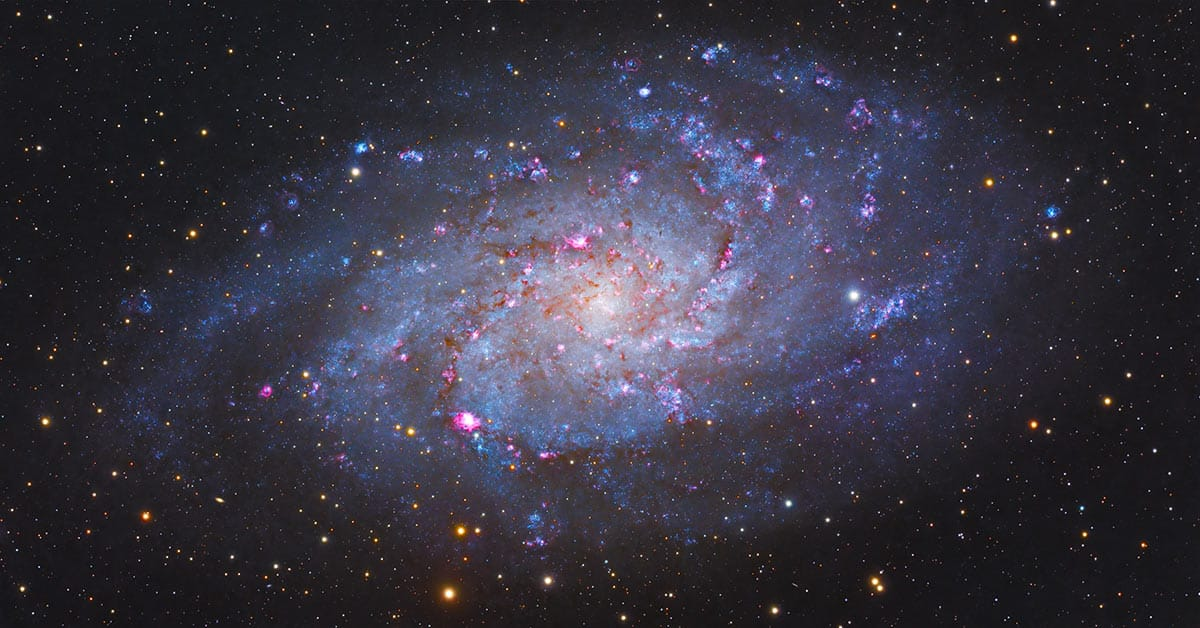
\includegraphics[width=1\linewidth]{files/triangulum-6481214de20cda52c86e4ba5076d2476.jpg}
\end{figure}

\subsubsection{Visão Geral}

O \textbf{Núcleo Triangulum} é responsável pela comunicação de profundidade e autoridade científica do Projeto Hermathena. Seu nome evoca a galáxia do Triângulo, símbolo de exploração profunda do cosmos, representando nosso compromisso com conteúdo aprofundado, documentários e produções que exigem tempo e expertise.

\subsubsection{Missão}

Produzir conteúdo audiovisual e jornalístico de alta qualidade que aprofunde o conhecimento científico sobre o BINGO e a cosmologia, estabelecendo o projeto como referência em divulgação científica no Brasil.

\subsubsection{Objetivos Específicos}

\paragraph{1. Podcasts e Áudio}

\subparagraph{1.1 ``RadioBingo'' - Podcast Principal}

\begin{itemize}
\item \textbf{Formato:} Notícias - Entrevista/Conteúdo Aprofundado
\item \textbf{Duração:} 20 minutos
\item \textbf{Frequência:} Quinzenal (2 episódios/mês)
\item \textbf{Plataformas:} Spotify, Apple Podcasts, Deezer, YouTube
\item \textbf{Estrutura:}

\begin{itemize}
\item Introdução (5 min) - Notícias da astronomia
\item Entrevista (13 min) - Tema aprofundado
\item Encerramento (2 min) - Próximos episódios e CTA
\end{itemize}
\end{itemize}

\subparagraph{1.2 ``BINGO Minuto'' - Micro-podcast}

\begin{itemize}
\item \textbf{Formato:} Notícias rápidas e curiosidades
\item \textbf{Duração:} 5-8 minutos
\item \textbf{Frequência:} Quinzenal
\item \textbf{Conteúdo:} Atualizações do projeto, explicações curtas, Notícias
\end{itemize}

\subparagraph{1.3 ``Mesa do Sertão'' - Conversas informais}

\begin{itemize}
\item \textbf{Formato:} Debates em mesa-redonda
\item \textbf{Duração:} 45 minutos
\item \textbf{Frequência:} Mensal
\item \textbf{Tema:} Ciência, cultura e desenvolvimento regional
\end{itemize}

\paragraph{2. Canal no YouTube}

\subparagraph{2.1 Séries de Conteúdo}

\textbf{Série ``Construindo o BINGO'' (Documental)}

\begin{itemize}
\item 12 episódios de 10-15 minutos
\item Acompanhamento da construção do telescópio
\item Entrevistas com engenheiros e técnicos
\item Lançamento: 1 episódio por mês
\end{itemize}

\textbf{Série ``Cosmologia para Todos'' (Educativa)}

\begin{itemize}
\item Vídeos de 8-12 minutos
\item Conceitos fundamentais explicados visualmente
\item Animações e infográficos
\item Frequência: 1 x por mês
\end{itemize}

\textbf{Série ``Pergunte ao Cientista'' (Q\&A)}

\begin{itemize}
\item Respostas em vídeo a perguntas do público
\item Duração: 5-10 minutos
\item Frequência: Semanal
\item Fonte: Perguntas das redes sociais
\end{itemize}

\subparagraph{2.2 Lives e Transmissões}

\bigskip\noindent
\begin{tabular}{p{\dimexpr 0.250\linewidth-2\tabcolsep}p{\dimexpr 0.250\linewidth-2\tabcolsep}p{\dimexpr 0.250\linewidth-2\tabcolsep}p{\dimexpr 0.250\linewidth-2\tabcolsep}}
\toprule
Evento & Frequência & Duração & Conteúdo \\
\hline
Live mensal & trimestral & 1 hora & Tema livre com Q\&A \\
Webinários técnicos & 2x/ano & 2 horas & Seminários científicos \\
Cobertura de eventos & Eventuais & Variável & Feiras, workshops, inaugurações \\
\bottomrule
\end{tabular}

\bigskip

\paragraph{3. Documentários}

\subparagraph{3.1 Documentário Principal: ``BINGO: Olhos no Sertão''}

\begin{itemize}
\item \textbf{Duração:} 45-60 minutos
\item \textbf{Formato:} Documentário científico
\item \textbf{Lançamento:} Final do primeiro ano
\item \textbf{Sinopse:} A história do primeiro radiotelescópio de grande porte do Brasil, desde sua concepção até as primeiras observações
\item \textbf{Distribuição:} YouTube, streaming educacional, TVs públicas
\end{itemize}

\subparagraph{3.2 Documentários Curtos (15 min)}

\bigskip\noindent
\begin{tabular}{p{\dimexpr 0.333\linewidth-2\tabcolsep}p{\dimexpr 0.333\linewidth-2\tabcolsep}p{\dimexpr 0.333\linewidth-2\tabcolsep}}
\toprule
Título & Tema & Prazo \\
\hline
``A Escolha do Sertão'' & Por que Aguiar foi escolhido & Mês 6 \\
``Engenheiros do Impossível'' & Desafios técnicos da construção & Mês 8 \\
``Olhando o Invisível'' & Como a radioastronomia funciona & Mês 10 \\
``O Futuro Começa Aqui'' & Impacto do BINGO para o Brasil & Mês 12 \\
\bottomrule
\end{tabular}

\bigskip

\paragraph{4. Webinários e Seminários}

\subparagraph{4.1 Ciclo de Palestras BINGO}

\begin{itemize}
\item \textbf{Frequência:} Mensal
\item \textbf{Formato:} Palestra online com Q\&A
\item \textbf{Público:} Estudantes e pesquisadores
\item \textbf{Palestrantes:} Membros da colaboração BINGO
\item \textbf{Temas sugeridos:}

\begin{itemize}
\item ``Introdução à Cosmologia''
\item ``Energia Escura: O Mistério do Universo''
\item ``Radioastronomia: Uma Nova Janela''
\item ``Os BAO e a Escala do Universo''
\item ``Tecnologia do BINGO''
\end{itemize}
\end{itemize}

\subparagraph{4.2 Seminário Anual de Divulgação Científica}

\begin{itemize}
\item \textbf{Frequência:} Anual
\item \textbf{Duração:} 2 dias
\item \textbf{Formato:} Híbrido (presencial e online)
\item \textbf{Público:} Educadores, comunicadores, estudantes
\item \textbf{Atividades:} Palestras, workshops, mostra de trabalhos
\end{itemize}

\paragraph{5. Jornalismo Científico}

\subparagraph{5.1 Artigos Especiais}

\textbf{Blog Hermathena}

\begin{itemize}
\item Artigos longos (1.500-3.000 palavras)
\item Profundidade científica acessível
\item Frequência: 2x por mês
\item Temas:

\begin{itemize}
\item ``A História das BAO''
\item ``O Telescópio que Veio da China''
\item ``Cientistas Paraibanos no BINGO''
\item ``O Legado do Radiotelescópio''
\end{itemize}
\end{itemize}

\subparagraph{5.2 Reportagens}

\begin{itemize}
\item Cobertura jornalística de eventos
\item Entrevistas exclusivas com cientistas internacionais
\item Reportagens especiais para veículos de comunicação parceiros
\end{itemize}

\subsubsection{Estrutura de Produção}

\paragraph{Estúdio Mínimo Necessário}

\bigskip\noindent
\begin{tabular}{p{\dimexpr 0.333\linewidth-2\tabcolsep}p{\dimexpr 0.333\linewidth-2\tabcolsep}p{\dimexpr 0.333\linewidth-2\tabcolsep}}
\toprule
Equipamento & Especificação & Finalidade \\
\hline
\textbf{Câmera principal} & Sony ZV-E10 ou similar & Gravação de vídeo \\
\textbf{Lentes} & 16-50mm f/3.5-5.6 + 50mm f/1.8 & Versatilidade e baixa luz \\
\textbf{Microfone principal} & Tascam TM-70 ou similar & Áudio de qualidade \\
\textbf{Mixer áudio} & Tascam Mixcast 4 & Podcasts e lives \\
\textbf{Iluminação} & Kit softbox LED 3 pontos & Iluminação controlada \\
\textbf{Tripé} & Tripé profissional + gimbal & Estabilidade \\
\textbf{Fones} & Tascam TH-05 ou similar & Monitoramento \\
\textbf{Gravador portátil} & Zoom H1n & Entrevistas em campo \\
\bottomrule
\end{tabular}

\bigskip

\paragraph{Software de Produção}

\bigskip\noindent
\begin{tabular}{p{\dimexpr 0.333\linewidth-2\tabcolsep}p{\dimexpr 0.333\linewidth-2\tabcolsep}p{\dimexpr 0.333\linewidth-2\tabcolsep}}
\toprule
Categoria & Ferramenta & Uso \\
\hline
Edição de vídeo & Adobe Premiere Pro & Montagem final \\
Edição de áudio & Adobe Audition & Pós-produção sonora \\
Motion graphics & After Effects & Animações e vinhetas \\
Color grading & DaVinci Resolve & Correção de cor \\
Design gráfico & Photoshop/Illustrator & Thumbnails e artes \\
Gestão de projetos & Notion/Trello & Organização \\
\bottomrule
\end{tabular}

\bigskip

\paragraph{Fluxo de Produção de Documentário}

\begin{verbatim}
┌─────────────────┐    ┌─────────────────┐    ┌─────────────────┐
│ 1. PRÉ -PRODUÇÃO │ -> │ 2. PRODUÇÃO     │ -> │ 3. PÓS -PRODUÇÃO │
│                 │    │                 │    │                 │
│ \cdot Pesquisa      │    │ \cdot Filmagens     │    │ \cdot Edição        │
│ \cdot Roteiro       │    │ \cdot Entrevistas   │    │ \cdot Áudio         │
│ \cdot Planejamento  │    │ \cdot B -roll        │    │ \cdot Finalização   │
│ \cdot Permissões    │    │ \cdot Áudio         │    │ \cdot Legendas      │
└─────────────────┘    └─────────────────┘    └─────────────────┘
        │                                              │
        v                                              v
┌─────────────────┐                         ┌─────────────────┐
│ 4. REVISÃO      │ < -                      │ 5. DISTRIBUIÇÃO │
│                 │                         │                 │
| \cdot Validação     │                         │ \cdot YouTube       │
│   científica    │                         │ \cdot Podcasts      │
| \cdot Ajustes       │                         │ \cdot Imprensa      │
└─────────────────┘                         └─────────────────┘
\end{verbatim}

\subsubsection{Cronograma de Produção (Ano 1)}

\paragraph{Trimestre 1: Setup e Primeiras Produções}

\bigskip\noindent
\begin{tabular}{p{\dimexpr 0.333\linewidth-2\tabcolsep}p{\dimexpr 0.333\linewidth-2\tabcolsep}p{\dimexpr 0.333\linewidth-2\tabcolsep}}
\toprule
Semana & Atividade & Entregável \\
\hline
1-2 & Aquisição e setup de equipamentos & Estúdio funcional \\
3-4 & Testes e gravações piloto & Episódios pilotos \\
5-6 & Lançamento podcast ``Cosmos em Foco'' & 2 episódios no ar \\
7-8 & Lançamento canal YouTube & 4 vídeos publicados \\
9-10 & Primeiras lives & 2 transmissões \\
11-12 & Análise e ajustes & Relatório de aprendizados \\
\bottomrule
\end{tabular}

\bigskip

\paragraph{Trimestre 2-4: Consolidação}

\bigskip\noindent
\begin{tabular}{p{\dimexpr 0.333\linewidth-2\tabcolsep}p{\dimexpr 0.333\linewidth-2\tabcolsep}p{\dimexpr 0.333\linewidth-2\tabcolsep}}
\toprule
Trimestre & Foco & Meta \\
\hline
\textbf{T2} & Consolidação de formatos & 6 episódios podcast, 12 vídeos \\
\textbf{T3} & Expansão de conteúdo & Webinários, parcerias \\
\textbf{T4} & Documentário principal & Finalização e lançamento \\
\bottomrule
\end{tabular}

\bigskip

\subsubsection{Métricas de Sucesso}

\paragraph{Indicadores Quantitativos}

\bigskip\noindent
\begin{tabular}{p{\dimexpr 0.333\linewidth-2\tabcolsep}p{\dimexpr 0.333\linewidth-2\tabcolsep}p{\dimexpr 0.333\linewidth-2\tabcolsep}}
\toprule
Plataforma & Indicador & Meta Ano 1 \\
\hline
Spotify & Downloads mensais & 500 \\
YouTube & Inscritos & 2.000 \\
YouTube & Visualizações/mês & 5.000 \\
YouTube & Horas de exibição & 500/mês \\
Lives & Espectadores simultâneos & 100 \\
Blog & Visitas/mês & 1.000 \\
\bottomrule
\end{tabular}

\bigskip

\paragraph{Indicadores Qualitativos}

\begin{itemize}
\item \textbf{Retenção de audiência:} \textgreater 50\% do vídeo assistido
\item \textbf{Comentários qualificados:} Perguntas e debates significativos
\item \textbf{Citações em mídia:} Referências ao conteúdo produzido
\item \textbf{Engajamento educacional:} Uso em sala de aula
\end{itemize}

\subsubsection{Parcerias de Conteúdo}

\paragraph{Institucionais}

\bigskip\noindent
\begin{tabular}{p{\dimexpr 0.333\linewidth-2\tabcolsep}p{\dimexpr 0.333\linewidth-2\tabcolsep}p{\dimexpr 0.333\linewidth-2\tabcolsep}}
\toprule
Parceiro & Tipo de Parceria & Contribuição \\
\hline
USP/INPE & Entrevistados & Cientistas para podcasts \\
UEPB/UFPB & Co-produção & Conteúdo regional \\
TVs Universitárias & Distribuição & Exibição de documentários \\
Rádios locais & Áudio & Transmissão de podcasts \\
\bottomrule
\end{tabular}

\bigskip

\paragraph{Comerciais}

\bigskip\noindent
\begin{tabular}{p{\dimexpr 0.333\linewidth-2\tabcolsep}p{\dimexpr 0.333\linewidth-2\tabcolsep}p{\dimexpr 0.333\linewidth-2\tabcolsep}}
\toprule
Parceiro & Tipo & Benefício \\
\hline
Spotify & Plataforma & Distribuição \\
YouTube & Plataforma & Monetização futura \\
Padlet/Escolas & Distribuição & Alcance educacional \\
\bottomrule
\end{tabular}

\bigskip

\subsubsection{Estrutura da Equipe}

\bigskip\noindent
\begin{tabular}{p{\dimexpr 0.333\linewidth-2\tabcolsep}p{\dimexpr 0.333\linewidth-2\tabcolsep}p{\dimexpr 0.333\linewidth-2\tabcolsep}}
\toprule
Função & Quantidade & Perfil \\
\hline
\textbf{Professor Orientador} & 1 & Docente Comunicação/Cinema \\
\textbf{Professor Colaborador} & 1 & Docente área complementar \\
\textbf{Bolsista PROBEX} & 1 & Graduação Comunicação/Cinema \\
\textbf{Voluntários} & 5 & Graduação em áreas afins \\
\bottomrule
\end{tabular}

\bigskip

\textbf{Total por núcleo:} 8 pessoas

\textbf{Expansão:} Pode replicar em instituições parceiras (até 12 alunos + 4 docentes)

\subsubsection{Orçamento Estimado (Ano 1)}

\bigskip\noindent
\begin{tabular}{p{\dimexpr 0.500\linewidth-2\tabcolsep}p{\dimexpr 0.500\linewidth-2\tabcolsep}}
\toprule
Categoria & Valor (R\$) \\
\hline
Bolsa (1 bolsista $\times$ 6 meses $\times$ R\$ 400) & 2.400,00 \\
Equipamentos (câmera, áudio, iluminação) & 20.000,00 \\
Software e assinaturas & 3.000,00 \\
Produção de documentário & 8.000,00 \\
Deslocamentos para gravações & 5.000,00 \\
Infraestrutura de estúdio & 4.000,00 \\
\textbf{Total} & \textbf{48.400,00} \\
\bottomrule
\end{tabular}

\bigskip

\subsubsection{Referências e Benchmarking}

\paragraph{Canais de Referência}

\bigskip\noindent
\begin{tabular}{p{\dimexpr 0.333\linewidth-2\tabcolsep}p{\dimexpr 0.333\linewidth-2\tabcolsep}p{\dimexpr 0.333\linewidth-2\tabcolsep}}
\toprule
Canal & Plataforma & O que aprender \\
\hline
Canal do Pirulla & YouTube & Divulgação científica acessível \\
SciShow & YouTube & Produção ágil e consistente \\
RadioLab & Podcast & Narrativa sonora \\
Nerdologia & YouTube & Hibridização cultura pop + ciência \\
Space Today & YouTube & Cobertura de astronomia \\
Vox & YouTube & Produção visual de alta qualidade \\
\bottomrule
\end{tabular}

\bigskip


\bigskip
\centerline{\rule{13cm}{0.4pt}}
\bigskip

\textit{Documento sujeito a ajustes conforme evolução da produção.}

\subsection{Núcleo Via Láctea: Comunicação Institucional e Educacional}

\begin{figure}[!htbp]
\centering
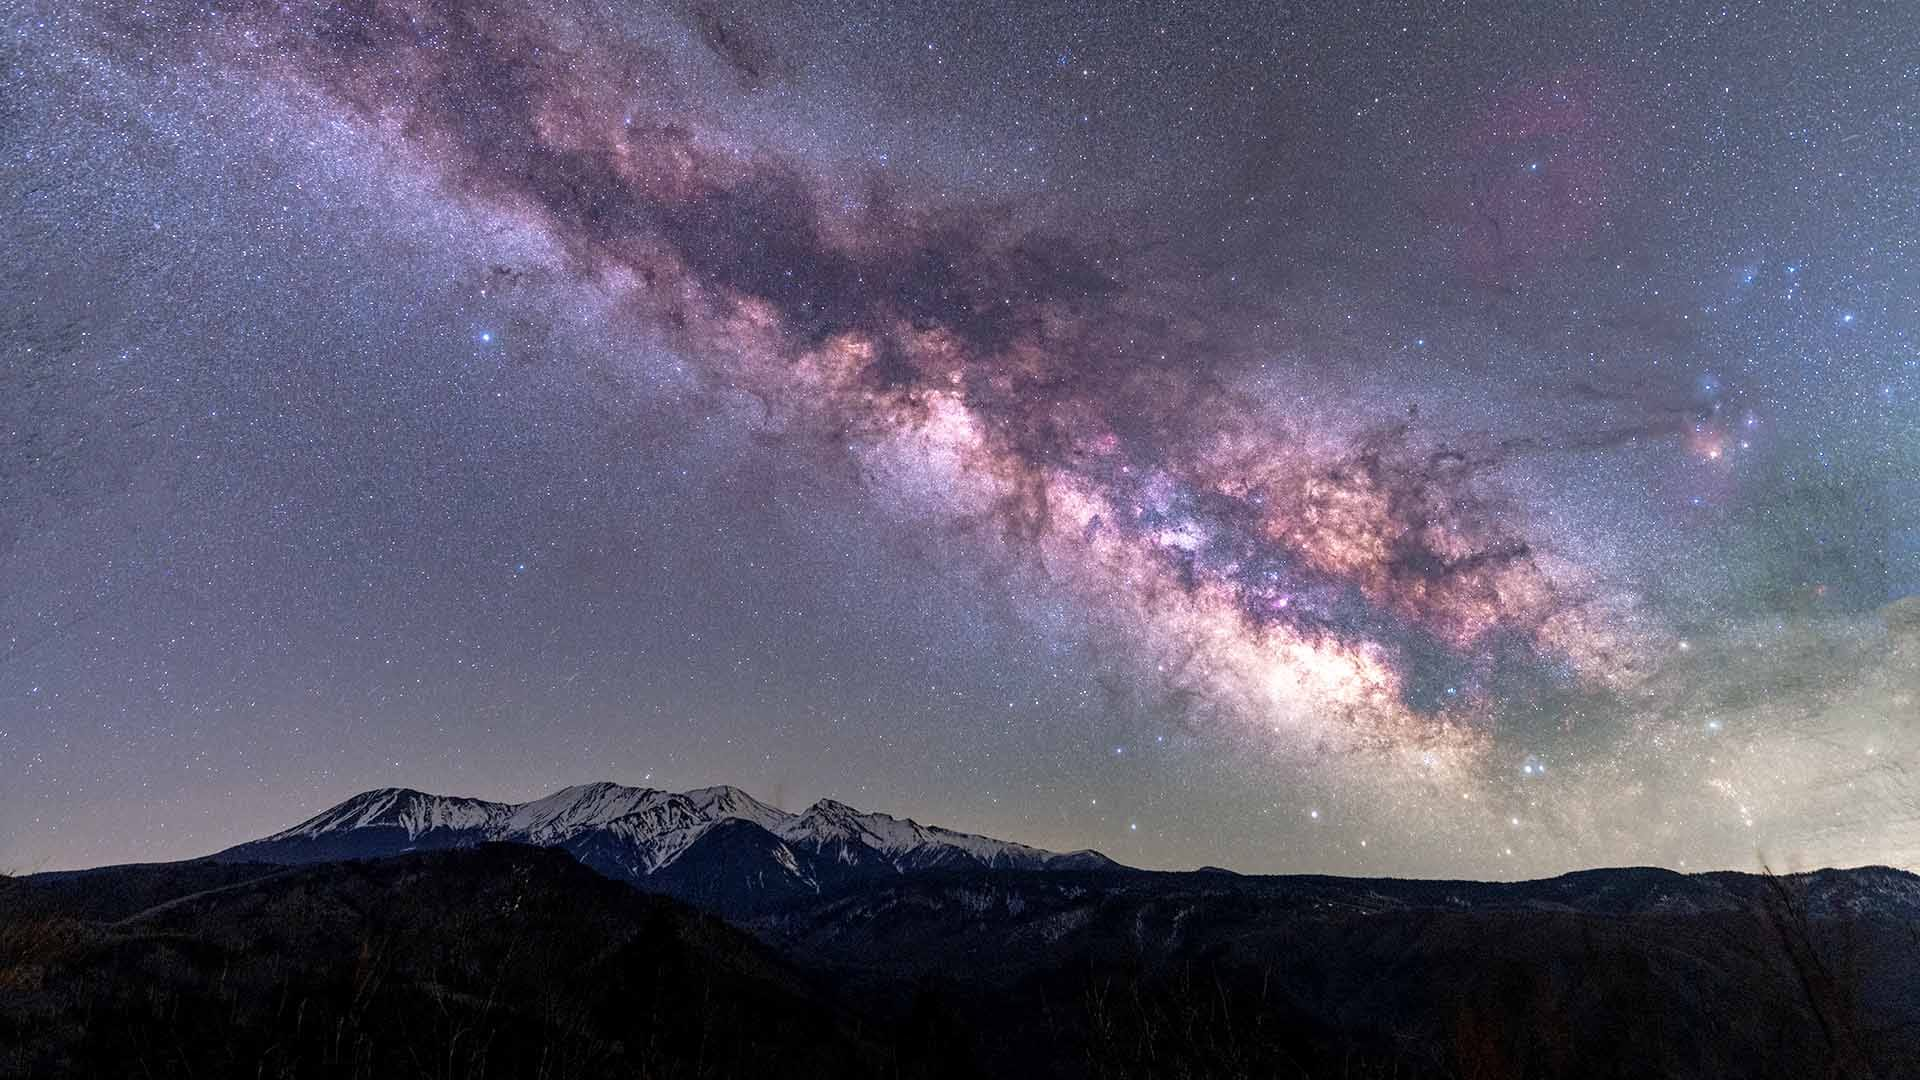
\includegraphics[width=1\linewidth]{files/vialactea-241d9e214ff4a2bcd2fd28d88f547093.jpg}
\end{figure}

\subsubsection{Visão Geral}

O \textbf{Núcleo Via Láctea} é responsável pelas ações de comunicação institucional e educacional do Projeto Hermathena. Seu nome evoca a nossa galáxia, simbolizando a base sólida sobre a qual se constrói toda a comunicação do projeto.

\subsubsection{Missão}

Estabelecer a identidade e a presença institucional do BINGO, produzir conteúdo educacional de qualidade e articular parcerias estratégicas com instituições formais.

\subsubsection{Objetivos Específicos}

\paragraph{1. Comunicação Institucional}

\subparagraph{1.1 Portal Web}

\begin{itemize}
\item[$\square$] Consolidar o portal \href{http://bingotelescope.org}{bingotelescope.org} como central de conteúdos
\item[$\square$] Implementar seção dedicada ao público brasileiro
\item[$\square$] Criar área de downloads para materiais educacionais
\item[$\square$] Estabelecer sistema de newsletter
\end{itemize}

\subparagraph{1.2 Identidade Visual}

\begin{itemize}
\item[$\square$] Desenvolver manual de identidade visual do Projeto Hermathena
\item[$\square$] Criar templates para documentos oficiais
\item[$\square$] Padronizar presença em eventos (banners, folders)
\item[$\square$] Implementar diretrizes de uso da marca BINGO
\end{itemize}

\subparagraph{1.3 Assessoria de Imprensa}

\begin{itemize}
\item[$\square$] Produzir press releases mensais
\item[$\square$] Manter banco de dados de jornalistas
\item[$\square$] Organizar coletivas de imprensa
\item[$\square$] Monitorar clipping de mídia
\end{itemize}

\paragraph{2. Comunicação Educacional}

\subparagraph{2.1 Material Didático}

\textbf{Para Ensino Fundamental (anos finais):}

\begin{itemize}
\item Cartilha ``O Universo em suas Mãos''
\item Jogos educativos sobre Sistema Solar
\item Posters astronômicos para sala de aula
\item Atividades práticas com materiais simples
\end{itemize}

\textbf{Para Ensino Médio:}

\begin{itemize}
\item Manual de Radioastronomia Básica
\item Roteiros de observação astronômica
\item Simulações computacionais
\item Propostas de experimentos
\end{itemize}

\textbf{Para Educadores:}

\begin{itemize}
\item Guia do Professor
\item Roteiros de aula estruturados
\item Sugestões de avaliação
\item Formação continuada
\end{itemize}

\subparagraph{2.2 Equipamentos de Demonstração}

\bigskip\noindent
\begin{tabular}{p{\dimexpr 0.333\linewidth-2\tabcolsep}p{\dimexpr 0.333\linewidth-2\tabcolsep}p{\dimexpr 0.333\linewidth-2\tabcolsep}}
\toprule
Equipamento & Descrição & Público-alvo \\
\hline
\textbf{Maquete do BINGO} & Modelo em escala 1:100 & Todos \\
\textbf{Radiolescópio didático} & Receptor de FM modificado & Ensino Médio \\
\textbf{Antena Hidrogeniana} & Receptor da linha de 21cm & Cursos técnicos \\
\textbf{Simulador de BAO} & Visualização de oscilações & Graduação \\
\textbf{Planetário portátil} & Projeção de constelações & Fundamental \\
\bottomrule
\end{tabular}

\bigskip

\subparagraph{2.3 Visitas e Experiências}

\begin{itemize}
\item \textbf{Visitas guiadas ao BINGO:} Protocolo de recebimento de escolas
\item \textbf{Roteiros de experiência:} Vivências práticas em radioastronomia
\item \textbf{Feiras de ciências:} Participação em eventos regionais
\item \textbf{Observações astronômicas:} Eventos noturnos com telescópios ópticos
\end{itemize}

\paragraph{3. Articulação Institucional}

\subparagraph{3.1 Parcerias Acadêmicas}

\bigskip\noindent
\begin{tabular}{p{\dimexpr 0.333\linewidth-2\tabcolsep}p{\dimexpr 0.333\linewidth-2\tabcolsep}p{\dimexpr 0.333\linewidth-2\tabcolsep}}
\toprule
Instituição & Tipo de Parceria & Ações Previstas \\
\hline
UEPB & Cooperação técnica & Divulgação no interior \\
IFPB & Cooperação técnica & Formação técnica \\
UFPB & Cooperação técnica & Pesquisa e extensão \\
USP & Colaboração BINGO & Suporte científico \\
INPE & Colaboração BINGO & Infraestrutura \\
\bottomrule
\end{tabular}

\bigskip

\subparagraph{3.2 Parcerias Governamentais}

\begin{itemize}
\item \textbf{SEECT-PB:} Integração com políticas estaduais de C\&T
\item \textbf{FAPESQ:} Cooperação em divulgação científica
\item \textbf{Prefeituras:} Ações em escolas municipais
\item \textbf{Secretarias de Educação:} Incorporação ao currículo
\end{itemize}

\subparagraph{3.3 Parcerias Privadas}

\begin{itemize}
\item Modelos: Patrocínio, mecenato, cooperação técnica
\item Setores prioritários: Telecom, energia, EdTech, turismo
\item Propostas personalizadas por segmento
\end{itemize}

\subsubsection{Metodologia}

\paragraph{Abordagem Educomunicativa}

Baseada nos princípios de:

\begin{enumerate}
\item \textbf{Diálogo horizontal:} Ciência como conversa, não imposição
\item \textbf{Contextualização:} Conectar conteúdo à realidade local
\item \textbf{Experimentação:} Aprender fazendo
\item \textbf{Colaboração:} Trabalho em rede
\end{enumerate}

\paragraph{Processo de Produção de Material}

\begin{verbatim}
┌─────────────┐    ┌─────────────┐    ┌─────────────┐    ┌─────────────┐
│  1. PESQUISA │ -> │ 2. ROTEIRO  │ -> │ 3. PRODUÇÃO │ -> │ 4. REVISÃO  │
│             │    │             │    │             │    │             │
│ Análise de  │    │ Estruturação│    │ Criação de  │    │ Validação   │
│ necessidades│    │ do conteúdo │    │ peças       │    │ com público │
└─────────────┘    └─────────────┘    └─────────────┘    └─────────────┘
                                                                │
                                                                v
┌─────────────┐    ┌─────────────┐    ┌─────────────┐    ┌─────────────┐
│ 8. ATUALIZA │ < - │ 7. AVALIAÇÃO│ < - │ 6. DIFUSÃO  │ < - │ 5. PUBLICAÇÃO│
│             │    │             │    │             │    │             │
│ Melhorias   │    │ Métricas de │    │ Distribuição│    │ Disponibili -│
│ contínuas   │    │ impacto     │    │ nos canais  │    │ zação formal│
└─────────────┘    └─────────────┘    └─────────────┘    └─────────────┘
\end{verbatim}

\subsubsection{Cronograma de Ações (Ano 1)}

\bigskip\noindent
\begin{tabular}{p{\dimexpr 0.250\linewidth-2\tabcolsep}p{\dimexpr 0.250\linewidth-2\tabcolsep}p{\dimexpr 0.250\linewidth-2\tabcolsep}p{\dimexpr 0.250\linewidth-2\tabcolsep}}
\toprule
Trimestre & Ação & Responsável & Produto \\
\hline
\textbf{T1} & Setup da infraestrutura & Coordenação & Estrutura operacional \\
\textbf{T1} & Desenvolvimento de identidade visual & Designer & Manual de marca \\
\textbf{T2} & Produção de material didático v1 & Equipe & 5 peças publicadas \\
\textbf{T2} & Primeiras visitas a escolas & Equipe & 3 escolas visitadas \\
\textbf{T3} & Workshop para educadores & Equipe & 20 participantes \\
\textbf{T3} & Feira de ciências regional & Equipe & Stand BINGO \\
\textbf{T4} & Avaliação e ajustes & Coordenação & Relatório de impacto \\
\bottomrule
\end{tabular}

\bigskip

\subsubsection{Indicadores}

\bigskip\noindent
\begin{tabular}{p{\dimexpr 0.333\linewidth-2\tabcolsep}p{\dimexpr 0.333\linewidth-2\tabcolsep}p{\dimexpr 0.333\linewidth-2\tabcolsep}}
\toprule
Indicador & Meta Ano 1 & Ferramenta de Medição \\
\hline
Materiais educacionais produzidos & 15 & Inventário \\
Escolas atendidas presencialmente & 10 & Registro de visitas \\
Educadores capacitados & 50 & Listas de presença \\
Downloads de materiais & 1.000 & Analytics \\
Parcerias institucionais firmadas & 5 & Acordos assinados \\
Releases publicados & 12 & Clipping \\
\bottomrule
\end{tabular}

\bigskip

\subsubsection{Estrutura da Equipe}

\bigskip\noindent
\begin{tabular}{p{\dimexpr 0.333\linewidth-2\tabcolsep}p{\dimexpr 0.333\linewidth-2\tabcolsep}p{\dimexpr 0.333\linewidth-2\tabcolsep}}
\toprule
Função & Quantidade & Perfil \\
\hline
\textbf{Professor Orientador} & 1 & Docente Física/Engenharia Elétrica \\
\textbf{Professor Colaborador} & 1 & Docente área complementar \\
\textbf{Bolsista PROBEX} & 1 & Graduação na área de afinidade \\
\textbf{Voluntários} & 5 & Graduação em áreas afins \\
\bottomrule
\end{tabular}

\bigskip

\textbf{Total por núcleo:} 8 pessoas

\textbf{Expansão:} Pode replicar em instituições parceiras (até 12 alunos + 4 docentes)

\subsubsection{Orçamento Estimado (Ano 1)}

\bigskip\noindent
\begin{tabular}{p{\dimexpr 0.500\linewidth-2\tabcolsep}p{\dimexpr 0.500\linewidth-2\tabcolsep}}
\toprule
Categoria & Valor (R\$) \\
\hline
Bolsa (1 bolsista $\times$ 6 meses $\times$ R\$ 400) & 2.400,00 \\
Material de consumo & 5.000,00 \\
Equipamentos de demonstração & 8.000,00 \\
Impressões gráficas & 3.000,00 \\
Deslocamentos & 5.000,00 \\
Eventos & 4.000,00 \\
\textbf{Total} & \textbf{33.400,00} \\
\bottomrule
\end{tabular}

\bigskip


\bigskip
\centerline{\rule{13cm}{0.4pt}}
\bigskip

\textit{Documento sujeito a revisões conforme evolução do projeto.}

\subsection{Núcleo Andromeda: Comunicação de Engajamento}

\begin{figure}[!htbp]
\centering
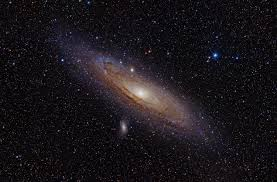
\includegraphics[width=1\linewidth]{files/andromeda-24292683f0310a3e603bd61d6d950606.jpeg}
\end{figure}

\subsubsection{Visão Geral}

O \textbf{Núcleo Andromeda} é responsável pela comunicação de engajamento digital do Projeto Hermathena. Seu nome evoca a galáxia vizinha, simbolizando a expansão e alcance da mensagem do BINGO através das redes sociais e canais digitais.

\subsubsection{Missão}

Criar conexões emocionais e intelectuais entre o público e o Radiotelescópio BINGO através de conteúdo digital criativo, acessível e viral, construindo uma comunidade online engajada em torno da ciência.

\subsubsection{Objetivos Específicos}

\paragraph{1. Gestão de Redes Sociais}

\subparagraph{1.1 Instagram}

\begin{itemize}
\item[$\square$] Criar e manter perfil oficial do Projeto Hermathena/BINGO PB
\item[$\square$] Publicar feed diário com conteúdo variado
\item[$\square$] Produzir Stories com interatividade (enquetes, caixinhas de perguntas)
\item[$\square$] Desenvolver Reels virais sobre astronomia e cosmologia
\item[$\square$] Alcançar 5.000 seguidores no primeiro ano
\item[$\square$] Manter taxa de engajamento superior a 5\%
\end{itemize}

\subparagraph{1.2 Facebook}

\begin{itemize}
\item[$\square$] Manter página institucional atualizada
\item[$\square$] Criar grupo de comunidade para educadores
\item[$\square$] Compartilhar eventos e lives
\item[$\square$] Publicar conteúdo em formato de álbum
\item[$\square$] Interagir com páginas de parceiros
\end{itemize}

\subparagraph{1.3 TikTok}

\begin{itemize}
\item[$\square$] Criar perfil com identidade jovem e descontraída
\item[$\square$] Produzir vídeos curtos (15-60 segundos)
\item[$\square$] Participar de trends educativas
\item[$\square$] Criar desafios de ciência
\item[$\square$] Colaborar com criadores de conteúdo da região
\end{itemize}

\paragraph{2. Estratégias de Conteúdo}

\subparagraph{2.1 Formatos por Plataforma}

\bigskip\noindent
\begin{tabular}{p{\dimexpr 0.250\linewidth-2\tabcolsep}p{\dimexpr 0.250\linewidth-2\tabcolsep}p{\dimexpr 0.250\linewidth-2\tabcolsep}p{\dimexpr 0.250\linewidth-2\tabcolsep}}
\toprule
Plataforma & Formato Principal & Frequência & Tom \\
\hline
Instagram & Carrossel educativo & Semanal & Inspirador \\
Instagram & Reels & Semanal & Entretenimento \\
Stories & Interativo & Semanal & Conversacional \\
Facebook & Posts longos & Semanal & Informativo \\
TikTok & Vídeos curtos & Semanal & Descontraído \\
\bottomrule
\end{tabular}

\bigskip

\subparagraph{2.2 Linhas Editoriais}

\textbf{\#CosmoEm60Segundos}

\begin{itemize}
\item Explicações rápidas de conceitos astronômicos
\item Curiosidades do universo
\item Respostas a perguntas do público
\end{itemize}

\textbf{\#BINGONoDetalhe}

\begin{itemize}
\item Bastidores da construção do telescópio
\item Entrevistas com técnicos e engenheiros
\item Mostra de equipamentos e tecnologia
\end{itemize}

\textbf{\#ParaibaNoEspaco}

\begin{itemize}
\item Conexão entre o Sertão e a cosmologia
\item Histórias de pessoas do projeto
\item Beleza do Vale do Piancó
\end{itemize}

\textbf{\#DesafioSTEM}

\begin{itemize}
\item Experimentos caseiros de ciência
\item Desafios para estudantes
\item Quiz e perguntas interativas
\end{itemize}

\textbf{\#CienciaNaPratica}

\begin{itemize}
\item Vídeos de demonstrações
\item Lives de observação astronômica
\item Eventos em tempo real
\end{itemize}

\paragraph{3. Produção de Conteúdo Viral}

\subparagraph{3.1 Biblioteca de Conteúdo}

\bigskip\noindent
\begin{tabular}{p{\dimexpr 0.333\linewidth-2\tabcolsep}p{\dimexpr 0.333\linewidth-2\tabcolsep}p{\dimexpr 0.333\linewidth-2\tabcolsep}}
\toprule
Tipo & Quantidade Anual & Exemplos \\
\hline
Infográficos & 12 & ``O que são BAO?'', ``Escala do Universo'' \\
Vídeos curtos & 50 & Reels, TikToks, Shorts \\
Memes educativos & 30 & Astronomia em formato humor \\
\bottomrule
\end{tabular}

\bigskip

\subparagraph{3.2 Série Regular ``BINGO Responde''}

Formato: Vídeos curtos respondendo perguntas do público

\begin{itemize}
\item Duração: 30-60 segundos
\item Frequência: Semanal
\item Call-to-action: ``Mande sua pergunta nos comentários''
\end{itemize}

\paragraph{4. Engajamento Comunitário}

\subparagraph{4.1 Estratégias de Interação}

\begin{itemize}
\item \textbf{Responder todos os comentários} em até 12 horas
\item \textbf{Compartilhar posts de seguidores} que mencionarem o projeto
\item \textbf{Criar desafios mensais} com premiação simbólica
\item \textbf{Live quinzenal} com especialistas (colaboração com Núcleo Triangulum)
\end{itemize}

\subparagraph{4.2 Parcerias com Influenciadores}

\bigskip\noindent
\begin{tabular}{p{\dimexpr 0.333\linewidth-2\tabcolsep}p{\dimexpr 0.333\linewidth-2\tabcolsep}p{\dimexpr 0.333\linewidth-2\tabcolsep}}
\toprule
Categoria & Perfil & Ação \\
\hline
Educação & Professores de ciências & Divulgação em sala \\
Lifestyle & Criadores da Paraíba & Visita ao BINGO \\
Ciência & Divulgadores científicos & Colaboração de conteúdo \\
Local & Prefeituras da região & Alcance institucional \\
\bottomrule
\end{tabular}

\bigskip

\paragraph{5. Monitoramento e Métricas}

\subparagraph{5.1 KPIs Principais}

\bigskip\noindent
\begin{tabular}{p{\dimexpr 0.333\linewidth-2\tabcolsep}p{\dimexpr 0.333\linewidth-2\tabcolsep}p{\dimexpr 0.333\linewidth-2\tabcolsep}}
\toprule
Indicador & Meta Ano 1 & Ferramenta \\
\hline
Seguidores Instagram & 5.000 & Insights nativo \\
Seguidores TikTok & 3.000 & TikTok Analytics \\
Taxa de engajamento & \textgreater 5\% & Metricool/Sprout \\
Alcance mensal & 100.000 & Meta Business \\
Compartilhamentos & 1.000/mês & Analytics \\
Saves (Instagram) & 500/mês & Insights nativo \\
\bottomrule
\end{tabular}

\bigskip

\subparagraph{5.2 Relatórios}

\begin{itemize}
\item \textbf{Semanal:} Métricas rápidas de performance
\item \textbf{Mensal:} Análise detalhada com insights
\item \textbf{Trimestral:} Relatório completo para coordenação
\end{itemize}

\subparagraph{5.3 Ferramentas de Gestão}

\begin{itemize}
\item \textbf{Agendamento:} Metricool ou Later
\item \textbf{Design:} Canva Pro + Adobe Creative Cloud
\item \textbf{Edição de vídeo:} CapCut + Premiere Pro
\item \textbf{Analytics:} Meta Business Suite, TikTok Analytics
\end{itemize}

\subsubsection{Metodologia}

\paragraph{Fluxo de Produção de Conteúdo}

\begin{verbatim}
flowchart LR

A["Planejamento"]
B["Produção"]
C["Agendamento"]
E["Publicação"]
D["Análise"]

A - -> B - -> C
C - -> E
E - -> D
D - -> A

classDef p fill:#ff9a6e,color:white;
classDef prod fill:#F54927,color:white;
classDef exec fill:#c53a1f,color:white;
classDef anal fill:#8e2415,color:white;

class A p
class B,C prod
class E exec
class D anal
\end{verbatim}

\paragraph{Processo de Criação}

\begin{enumerate}
\item \textbf{Briefing} - Definição de objetivo, público e formato
\item \textbf{Pesquisa} - Verificação de dados científicos
\item \textbf{Roteirização} - Texto e estrutura visual
\item \textbf{Produção} - Design e edição
\item \textbf{Revisão} - Validação com equipe científica
\item \textbf{Aprovação} - Coordenação final
\item \textbf{Publicação} - Postagem otimizada
\item \textbf{Monitoramento} - Acompanhamento de performance
\end{enumerate}

\subsubsection{Cronograma de Ações (Ano 1)}

\bigskip\noindent
\begin{tabular}{p{\dimexpr 0.250\linewidth-2\tabcolsep}p{\dimexpr 0.250\linewidth-2\tabcolsep}p{\dimexpr 0.250\linewidth-2\tabcolsep}p{\dimexpr 0.250\linewidth-2\tabcolsep}}
\toprule
Trimestre & Ação & Responsável & Produto \\
\hline
\textbf{T1} & Setup dos perfis & Equipe & Perfis criados e configurados \\
\textbf{T1} & Definição de identidade visual digital & Designer & Guia de uso em redes sociais \\
\textbf{T2} & Produção de 30 posts iniciais & Equipe & Biblioteca de conteúdo \\
\textbf{T2} & Primeiras lives & Equipe & 4 transmissões ao vivo \\
\textbf{T3} & Campanha de crescimento & Equipe & Meta: 2.000 seguidores \\
\textbf{T3} & Parcerias com influencers & Coordenação & 3 colaborações \\
\textbf{T4} & Análise e otimização & Equipe & Relatório de melhores práticas \\
\textbf{T4} & Planejamento ano 2 & Coordenação & Calendário editorial anual \\
\bottomrule
\end{tabular}

\bigskip

\subsubsection{Campanhas Temáticas}

\paragraph{Calendário de Campanhas}

\bigskip\noindent
\begin{tabular}{p{\dimexpr 0.250\linewidth-2\tabcolsep}p{\dimexpr 0.250\linewidth-2\tabcolsep}p{\dimexpr 0.250\linewidth-2\tabcolsep}p{\dimexpr 0.250\linewidth-2\tabcolsep}}
\toprule
Mês & Campanha & Tema & Hashtag \\
\hline
Março & Dia da Astronomia & Mulheres na astronomia & \#MulheresNoBINGO \\
Abril & Semana da Terra & Terra e cosmologia & \#TerraNoCosmos \\
Maio & Dia do Astronauta & Exploração espacial & \#ParaibaNoEspaco \\
Junho & Dia do Meio Ambiente & Radioastronomia e preservação & \#BINGOVerde \\
Agosto & Dia do Estudante & Carreiras STEM & \#FuturoBINGO \\
Setembro & Semana Nacional de Ciência & Divulgação massiva & \#BINGOCiencia \\
Outubro & Dia das Crianças & Astronomia para pequenos & \#BINGOKids \\
Novembro & ENEM & Ciência na Escola & \#BINGOENEM \\
Dezembro & Retrospectiva & Melhores momentos do ano & \#BINGO2026 \\
\bottomrule
\end{tabular}

\bigskip

\subsubsection{Estrutura da Equipe}

\bigskip\noindent
\begin{tabular}{p{\dimexpr 0.333\linewidth-2\tabcolsep}p{\dimexpr 0.333\linewidth-2\tabcolsep}p{\dimexpr 0.333\linewidth-2\tabcolsep}}
\toprule
Função & Quantidade & Perfil \\
\hline
\textbf{Professor Orientador} & 1 & Docente Comunicação/Educomunicação \\
\textbf{Professor Colaborador} & 1 & Docente arte/mídia/jornalismo \\
\textbf{Bolsista PROBEX} & 1 & Graduação Comunicação/Jornalismo \\
\textbf{Voluntários} & 5 & Graduação em áreas afins \\
\bottomrule
\end{tabular}

\bigskip

\textbf{Total por núcleo:} 8 pessoas

\textbf{Expansão:} Pode replicar em instituições parceiras (até 12 alunos + 4 docentes)

\subsubsection{Orçamento Estimado (Ano 1)}

\bigskip\noindent
\begin{tabular}{p{\dimexpr 0.500\linewidth-2\tabcolsep}p{\dimexpr 0.500\linewidth-2\tabcolsep}}
\toprule
Categoria & Valor (R\$) \\
\hline
Bolsa (1 bolsista $\times$ 6 meses $\times$ R\$ 400) & 2.400,00 \\
Assinaturas de ferramentas & 3.600,00 \\
Equipamentos (ring light, tripé) & 2.000,00 \\
Eventos e parcerias & 3.000,00 \\
\textbf{Total} & \textbf{28.000,00} \\
\bottomrule
\end{tabular}

\bigskip

\subsubsection{Benchmarking}

\paragraph{Referências em Comunicação Científica Digital}

\bigskip\noindent
\begin{tabular}{p{\dimexpr 0.333\linewidth-2\tabcolsep}p{\dimexpr 0.333\linewidth-2\tabcolsep}p{\dimexpr 0.333\linewidth-2\tabcolsep}}
\toprule
Projeto & Plataforma & O que aprender \\
\hline
\cite{AstroPocket} & Instagram & Formato de carrossel educativo \\
\cite{CanalNostalgia} & YouTube/Instagram & Como viralizar ciência \\
NASA & Todas & Estratégia multicanal \\
IFScience & Facebook & Engajamento com conteúdo leve \\
Manual do Mundo & YouTube & Produção de vídeos didáticos \\
\bottomrule
\end{tabular}

\bigskip


\bigskip
\centerline{\rule{13cm}{0.4pt}}
\bigskip

\textit{Documento sujeito a revisões conforme evolução das plataformas digitais.}

\section{Estrategia}

\subsection{Abordagem Educomunicativa}

\subsubsection{Abordagem Educomunicativa}

\paragraph{Fundamentação Teórica}

\subparagraph{O que é Educomunicação?}

A \textbf{educomunicação} é um campo interdisciplinar que integra comunicação e educação, reconhecendo que:

\begin{quote}
\textit{``A comunicação é um processo educativo e a educação é um processo comunicativo''} --- Soares e Melo (2020)
\end{quote}

No Projeto Hermathena, adotamos a educomunicação como eixo central porque ela permite:

\begin{itemize}
\item \textbf{Diálogo horizontal} entre cientistas e público
\item \textbf{Construção conjunta} de conhecimento
\item \textbf{Contextualização} do conteúdo científico
\item \textbf{Empoderamento} dos participantes
\end{itemize}

\subparagraph{Três Vertentes Teóricas}

\begin{verbatim}
┌─────────────────────────────────────────────────────────────┐
│                 FUNDAÇÃO TEÓRICA                           │
├─────────────────────────────────────────────────────────────┤
│                                                             │
│   ┌──────────────┐  ┌──────────────┐  ┌──────────────┐    │
│   │ Educomuni -   │  │ Comunicação  │  │ Desenvolvi -  │    │
│   │ cação        │  │ Pública da   │  │ mento        │    │
│   │              │  │ Ciência      │  │ Regional     │    │
│   └──────┬───────┘  └──────┬───────┘  └──────┬───────┘    │
│          │                 │                 │             │
│          └─────────────────┼─────────────────┘             │
│                            │                               │
│                            ▼                               │
│                 ┌──────────────────────┐                   │
│                 │  PROJETO HERMATHENA  │                   │
│                 └──────────────────────┘                   │
│                                                             │
└─────────────────────────────────────────────────────────────┘
\end{verbatim}


\bigskip
\centerline{\rule{13cm}{0.4pt}}
\bigskip

\paragraph{1. Educomunicação}

\subparagraph{Princípios Fundamentais}

\subparagraph{1.1 Diálogo Horizontal}

Contrário ao modelo tradicional de transmissão de informação, propomos:

\bigskip\noindent
\begin{tabular}{p{\dimexpr 0.500\linewidth-2\tabcolsep}p{\dimexpr 0.500\linewidth-2\tabcolsep}}
\toprule
Modelo Tradicional & Modelo Educomunicativo \\
\hline
Cientista ensina & Cientista e público aprendem juntos \\
Conhecimento unidirecional & Troca de saberes \\
Público passivo & Público ativo e produtor \\
Linguagem técnica & Linguagem contextualizada \\
\bottomrule
\end{tabular}

\bigskip

\subparagraph{1.2 Processo Dialógico}

\begin{verbatim}
┌──────────────────────────────────────────────────────────────┐
│                     CICLO DIALÓGICO                         │
├──────────────────────────────────────────────────────────────┤
│                                                              │
│   ┌──────────┐      ┌──────────┐      ┌──────────┐         │
│   │  OUÇA    │ ───> │  DIALOGUE│ ───> │  CO -RIE  │         │
│   │          │      │          │      │          │         │
│   │ Entenda  │      │ Troque   │      │ Construa │         │
│   │ necessi - │      │ saberes  │      │ junto    │         │
│   │ dades    │      │          │      │          │         │
│   └──────────┘      └──────────┘      └────┬─────┘         │
│         ^                                   │               │
│         │                                   │               │
│         └───────────────────────────────────┘               │
│                        AVALIE                               │
│                                                              │
└──────────────────────────────────────────────────────────────┘
\end{verbatim}

\subparagraph{Aplicação no Projeto}

\textbf{Exemplo: Produção de Material Didático}

\begin{enumerate}
\item \textbf{Pesquisa participativa}

\begin{itemize}
\item Entrevistas com professores sobre necessidades
\item Oficinas com estudantes para entender interesses
\item Consulta a especialistas em educação
\end{itemize}


\item \textbf{Co-criação}

\begin{itemize}
\item Workshops de roteirização com educadores
\item Testes pilotos em sala de aula
\item Feedback contínuo
\end{itemize}


\item \textbf{Validação comunitária}

\begin{itemize}
\item Revisão por professores da rede pública
\item Ajustes baseados na realidade escolar
\item Aprovação por equipe científica
\end{itemize}
\end{enumerate}


\bigskip
\centerline{\rule{13cm}{0.4pt}}
\bigskip

\paragraph{2. Comunicação Pública da Ciência}

\subparagraph{Modelo de Diálogo entre Iguais}

Segundo Irwin (2008), a comunicação pública da ciência evoluiu:

\bigskip\noindent
\begin{tabular}{p{\dimexpr 0.333\linewidth-2\tabcolsep}p{\dimexpr 0.333\linewidth-2\tabcolsep}p{\dimexpr 0.333\linewidth-2\tabcolsep}}
\toprule
Modelo & Característica & Era \\
\hline
\textbf{Deficitário} & ``O público precisa ser educado'' & 1950-1980 \\
\textbf{Diálogo} & ``Troca de perspectivas'' & 1990-2010 \\
\textbf{Participativo} & ``Ciência com e para a sociedade'' & 2010-presente \\
\bottomrule
\end{tabular}

\bigskip

\subparagraph{Abordagem do Hermathena: Modelo Participativo}

Características:

\begin{itemize}
\item \textbf{Reconhecimento de expertise local}: A comunidade tem saberes legítimos
\item \textbf{Transparência científica}: Divulgação de incertezas e limitações
\item \textbf{Deliberação pública}: Espaço para questionamentos
\item \textbf{Responsividade}: Ciência responde às demandas sociais
\end{itemize}

\subparagraph{Estratégias de Implementação}

\subparagraph{2.1 Ciência em Contexto}

Conectar o conteúdo à realidade do Sertão paraibano:

\bigskip\noindent
\begin{tabular}{p{\dimexpr 0.500\linewidth-2\tabcolsep}p{\dimexpr 0.500\linewidth-2\tabcolsep}}
\toprule
Tema Científico & Conexão Local \\
\hline
Energia escura & A ``força invisível'' como metáfora para o desenvolvimento regional \\
Radioastronomia & Tecnologia aplicada à agricultura (sensores) \\
BAO e escala cósmica & A escala do Sertão para o Brasil e mundo \\
Espectro eletromagnética & Comparação com comunicação por rádio local \\
\bottomrule
\end{tabular}

\bigskip

\subparagraph{2.2 Narrativas Inclusivas}

\begin{itemize}
\item Histórias de paraibanos na ciência
\item Reconhecimento de saberes tradicionais
\item Diálogo com cultura local (cordel, forró, arte sertaneja)
\end{itemize}


\bigskip
\centerline{\rule{13cm}{0.4pt}}
\bigskip

\paragraph{3. Desenvolvimento Regional}

\subparagraph{Ciência como Indutora de Desenvolvimento}

Segundo Lastres et al. (2005), a ciência e tecnologia funcionam como indutores de desenvolvimento quando:

\begin{itemize}
\item Articuladas com políticas públicas
\item Integradas à iniciativa privada
\item Apropriadas pela comunidade local
\end{itemize}

\subparagraph{O BINGO como Vetor de Desenvolvimento}

\begin{verbatim}
┌─────────────────────────────────────────────────────────────┐
│           IMPACTOS DO BINGO NA REGIÃO                       │
├─────────────────────────────────────────────────────────────┤
│                                                             │
│   ┌──────────────┐  ┌──────────────┐  ┌──────────────┐    │
│   │ HUMANO       │  │ CIENTÍFICO   │  │ ECONÔMICO    │    │
│   │              │  │              │  │              │    │
│   │ \cdot Formação   │  │ \cdot Pesquisa   │  │ \cdot Turismo    │    │
│   │   STEM       │  │   de ponta   │  │   científico │    │
│   │ \cdot Empoderam. │  │ \cdot Inovação   │  │ \cdot Inovação   │    │
│   │   comunitário│  │   tecnológica│  │   tecnológica│    │
│   └──────────────┘  └──────────────┘  └──────────────┘    │
│                                                             │
└─────────────────────────────────────────────────────────────┘
\end{verbatim}

\subparagraph{Comunicação como Facilitadora}

A comunicação científica do Hermathena potencializa esses impactos:

\begin{enumerate}
\item \textbf{Visibilidade nacional}: Atrai atenção e recursos para a região
\item \textbf{Educação de qualidade}: Prepara jovens para oportunidades
\item \textbf{Turismo científico}: Gera renda local
\item \textbf{Atração de investimentos}: Conecta empresas à ciência
\end{enumerate}


\bigskip
\centerline{\rule{13cm}{0.4pt}}
\bigskip

\paragraph{Metodologias Específicas}

\subparagraph{1. Design Instrucional}

\subparagraph{Análise de Necessidades (ADDIE)}

\begin{verbatim}
┌─────────┐   ┌─────────┐   ┌─────────┐   ┌─────────┐   ┌─────────┐
│ ANALISAR│ \rightarrow │  DESIGN │ \rightarrow │ DESENV. │ \rightarrow │IMPLEMENT│ \rightarrow │ AVALIAR │
└─────────┘   └─────────┘   └─────────┘   └─────────┘   └─────────┘
    │             │             │             │             │
    ▼             ▼             ▼             ▼             ▼
Perfil do    Objetivos    Produção     Aplicação   Métricas
devedor      de            do           em campo    de sucesso
             aprendizado   material
\end{verbatim}

\subparagraph{Aplicação}

\bigskip\noindent
\begin{tabular}{p{\dimexpr 0.500\linewidth-2\tabcolsep}p{\dimexpr 0.500\linewidth-2\tabcolsep}}
\toprule
Etapa & Ação no Hermathena \\
\hline
\textbf{Análise} & Pesquisa com 50 professores da rede pública \\
\textbf{Design} & Definição de objetivos por faixa etária \\
\textbf{Desenvolvimento} & Criação de materiais com equipe multidisciplinar \\
\textbf{Implementação} & Teste em 10 escolas piloto \\
\textbf{Avaliação} & Medição de aprendizado e satisfação \\
\bottomrule
\end{tabular}

\bigskip

\subparagraph{2. Produção Colaborativa}

\subparagraph{Modelo de Produção em Rede}

\begin{verbatim}
┌───────────────────┐
                    │   COORDENAÇÃO     │
                    │   HERMATHENA      │
                    └─────────┬─────────┘
                              │
        ┌─────────────────────┼─────────────────────┐
        │                     │                     │
        ▼                     ▼                     ▼
┌───────────────┐    ┌───────────────┐    ┌───────────────┐
│   ESCOLAS     │    │  UNIVERSIDADES│    │  COMUNIDADE   │
│               │    │               │    │               │
│ \cdot Professores │    │ \cdot Pesquisadores│   │ \cdot Lideranças  │
│ \cdot Estudantes  │    │ \cdot Graduandos  │    │ \cdot Artistas    │
│ \cdot Gestores    │    │ \cdot Pós -grad.   │    │ \cdot Empreended. │
└───────────────┘    └───────────────┘    └───────────────┘
\end{verbatim}

\subparagraph{3. Avaliação Participativa}

\subparagraph{Instrumentos}

\begin{enumerate}
\item \textbf{Pesquisa de Percepção Comunitária}

\begin{itemize}
\item Aplicação bianual
\item Amostra: 500 habitantes de Aguiar e região
\item Foco: Reconhecimento do BINGO, interesse em ciência
\end{itemize}


\item \textbf{Questionário de Satisfação}

\begin{itemize}
\item Pós-cada atividade
\item Escala Likert (1-5)
\item Espaço para sugestões abertas
\end{itemize}


\item \textbf{Grupos Focais}

\begin{itemize}
\item 2x por ano
\item 8-12 participantes
\item Discussão guiada sobre impacto
\end{itemize}


\item \textbf{Estudos de Caso}

\begin{itemize}
\item Narrativas individuais
\item Histórias de transformação
\item Documentação qualitativa
\end{itemize}
\end{enumerate}


\bigskip
\centerline{\rule{13cm}{0.4pt}}
\bigskip

\paragraph{Matriz de Conteúdos por Público}

\subparagraph{Ensino Fundamental (Anos Finais)}

\bigskip\noindent
\begin{tabular}{p{\dimexpr 0.333\linewidth-2\tabcolsep}p{\dimexpr 0.333\linewidth-2\tabcolsep}p{\dimexpr 0.333\linewidth-2\tabcolsep}}
\toprule
Tema & Abordagem & Produto \\
\hline
Sistema Solar & Jogos e atividades lúdicas & Cartilha ilustrada \\
Estrelas & Contação de histórias & Vídeos animados \\
Universo & Maquetes e modelos & Kit escolar \\
\bottomrule
\end{tabular}

\bigskip

\subparagraph{Ensino Médio}

\bigskip\noindent
\begin{tabular}{p{\dimexpr 0.333\linewidth-2\tabcolsep}p{\dimexpr 0.333\linewidth-2\tabcolsep}p{\dimexpr 0.333\linewidth-2\tabcolsep}}
\toprule
Tema & Abordagem & Produto \\
\hline
Cosmologia & Simulações computacionais & Software educativo \\
Radioastronomia & Experimentos práticos & Manual laboratorial \\
Método científico & Projetos de pesquisa & Guia do estudante \\
\bottomrule
\end{tabular}

\bigskip

\subparagraph{Educadores}

\bigskip\noindent
\begin{tabular}{p{\dimexpr 0.333\linewidth-2\tabcolsep}p{\dimexpr 0.333\linewidth-2\tabcolsep}p{\dimexpr 0.333\linewidth-2\tabcolsep}}
\toprule
Tema & Abordagem & Produto \\
\hline
Astronomia na sala & Formação continuada & Curso online \\
Uso de materiais didáticos & Oficinas práticas & Tutoriais em vídeo \\
Avaliação em ciências & Estudos de caso & Caderno de práticas \\
\bottomrule
\end{tabular}

\bigskip

\subparagraph{Público Geral}

\bigskip\noindent
\begin{tabular}{p{\dimexpr 0.333\linewidth-2\tabcolsep}p{\dimexpr 0.333\linewidth-2\tabcolsep}p{\dimexpr 0.333\linewidth-2\tabcolsep}}
\toprule
Tema & Abordagem & Produto \\
\hline
BINGO e a Paraíba & Documentários & Vídeos no YouTube \\
Curiosidades astronômicas & Redes sociais & Posts e reels \\
Ciência no cotidiano & Podcasts & Episódios mensais \\
\bottomrule
\end{tabular}

\bigskip


\bigskip
\centerline{\rule{13cm}{0.4pt}}
\bigskip

\paragraph{Cronograma Metodológico}

\subparagraph{Fase 1: Diagnóstico e Planejamento (Meses 1-2)}

\bigskip\noindent
\begin{tabular}{p{\dimexpr 0.333\linewidth-2\tabcolsep}p{\dimexpr 0.333\linewidth-2\tabcolsep}p{\dimexpr 0.333\linewidth-2\tabcolsep}}
\toprule
Semana & Atividade & Metodologia \\
\hline
1-2 & Pesquisa de campo com escolas & Entrevistas, questionários \\
3-4 & Análise de necessidades & Grupos focais \\
5-6 & Definição de matriz de conteúdos & Workshop participativo \\
7-8 & Planejamento pedagógico & Design instrucional \\
\bottomrule
\end{tabular}

\bigskip

\subparagraph{Fase 2: Produção e Testes (Meses 3-6)}

\bigskip\noindent
\begin{tabular}{p{\dimexpr 0.333\linewidth-2\tabcolsep}p{\dimexpr 0.333\linewidth-2\tabcolsep}p{\dimexpr 0.333\linewidth-2\tabcolsep}}
\toprule
Semana & Atividade & Metodologia \\
\hline
9-12 & Produção de materiais v1 & Co-criação com educadores \\
13-16 & Testes pilotos & Aplicação em 10 escolas \\
17-20 & Ajustes e refinamento & Análise de feedback \\
21-24 & Validação final & Comitê de especialistas \\
\bottomrule
\end{tabular}

\bigskip

\subparagraph{Fase 3: Implementação e Avaliação (Meses 7-12)}

\bigskip\noindent
\begin{tabular}{p{\dimexpr 0.333\linewidth-2\tabcolsep}p{\dimexpr 0.333\linewidth-2\tabcolsep}p{\dimexpr 0.333\linewidth-2\tabcolsep}}
\toprule
Semana & Atividade & Metodologia \\
\hline
25-32 & Implementação em larga escala & Ações nas escolas \\
33-40 & Monitoramento contínuo & Coleta de métricas \\
41-48 & Avaliação de impacto & Pesquisa de percepção \\
49-52 & Documentação e relatório & Análise de dados \\
\bottomrule
\end{tabular}

\bigskip


\bigskip
\centerline{\rule{13cm}{0.4pt}}
\bigskip

\paragraph{Referências}

\begin{itemize}
\item ALONSO, L. et al. \textit{A Educomunicação nos processos de educação e difusão de conhecimento: divulgação científica no Projeto Telescópio BINGO}. ECA-USP, 2023.
\item IRWIN, A. \textit{Risk, science and public communication}. In: The handbook of science and technology studies. 2008.
\item LASTRES, H. M. M.; CASSIOLATO, J. E.; ARROIO, A. (Org.). \textit{Conhecimento, sistemas de inovação e desenvolvimento}. Editora UFRJ, 2005.
\item SOARES, I. M. de M.; MELO, J. M. de. \textit{Educomunicação: conceitos e práticas}. Editora PUC-Rio, 2020.
\end{itemize}


\bigskip
\centerline{\rule{13cm}{0.4pt}}
\bigskip

\textit{Metodologia adaptável conforme aprendizados do projeto.}

\subsection{Estratégia Multicanal}

\subsubsection{Canais Digitais}

\paragraph{Estratégia Multicanal}

O Projeto Hermathena adota uma estratégia de comunicação multicanal, onde cada plataforma tem uma função específica no ecossistema de comunicação:

\begin{verbatim}
┌─────────────────────────────────────────────────────────────────┐
│                 ECOSISTEMA DIGITAL HERMATHENA                  │
├─────────────────────────────────────────────────────────────────┤
│                                                                 │
│                        ┌───────────┐                           │
│                        │  PORTAL   │                           │
│                        │   WEB     │ \leftarrow Central de conteúdo    │
│                        │  (Base)   │                           │
│                        └─────┬─────┘                           │
│                              │                                  │
│        ┌─────────────────────┼─────────────────────┐           │
│        │                     │                     │           │
│        ▼                     ▼                     ▼           │
│   ┌─────────┐          ┌─────────┐          ┌─────────┐       │
│   │ ENGAJAR │          │APROFUNDAR│          │ NOTIFICAR│       │
│   │         │          │         │          │         │       │
│   │Instagram│          │YouTube  │          │ Email   │       │
│   │ Facebook│          │Spotify  │          │ WhatsApp│       │
│   │ TikTok  │          │Blog     │          │         │       │
│   └─────────┘          └─────────┘          └─────────┘       │
│                                                                 │
└─────────────────────────────────────────────────────────────────┘
\end{verbatim}


\bigskip
\centerline{\rule{13cm}{0.4pt}}
\bigskip

\paragraph{1. Portal Web (\href{http://bingotelescope.org}{bingotelescope.org})}

\subparagraph{Função}

Central de conteúdo e repositório oficial de todos os materiais do projeto.

\subparagraph{Estrutura Proposta}

\begin{verbatim}
bingotelescope.org/
├── /
│   ├── Hero: O que é o BINGO
│   ├── Últimas notícias
│   ├── Próximos eventos
│   └── Chamada para ação (newsletter)
│
├── /sobre
│   ├── O projeto BINGO
│   ├── Colaboração internacional
│   ├── Equipe brasileira
│   └── Linha do tempo
│
├── /para -quem
│   ├── /estudantes (Fundamental, Médio)
│   ├── /educadores (Materiais didáticos)
│   ├── /pesquisadores (Publicações técnicas)
│   └── /publico -geral (Conteúdo acessível)
│
├── /noticias
│   ├── /tekoha (Notícias locais)
│   ├── /urania (Notícias gerais)
│   └── /guaraci (Institucional)
│
├── /eixos
│   ├── /tengre (Fundamental)
│   ├── /shiva -nataraja (Médio)
│   ├── /sun -wukong (Técnico)
│   └── /guaraci (Institucional)
│
├── /materiais
│   ├── Download de cartilhas
│   ├── Vídeos
│   ├── Podcasts
│   └── Infográficos
│
├── /visite
│   ├── Como chegar
│   ├── Agendamento de visitas
│   ├── Roteiros virtuais
│   └── FAQ
│
└── /contato
    ├── Formulário
    ├── Imprensa
    └── Parcerias
\end{verbatim}

\subparagraph{Funcionalidades}

\bigskip\noindent
\begin{tabular}{p{\dimexpr 0.333\linewidth-2\tabcolsep}p{\dimexpr 0.333\linewidth-2\tabcolsep}p{\dimexpr 0.333\linewidth-2\tabcolsep}}
\toprule
Funcionalidade & Descrição & Prioridade \\
\hline
Sistema de busca & Encontrar conteúdo por tema, faixa etária, formato & Alta \\
Newsletter & Cadastro para boletim quinzenal & Alta \\
Downloads & Materiais em PDF, vídeos & Alta \\
Agendamento & Sistema de marcação de visitas & Média \\
Blog & Artigos e notícias & Alta \\
Multilíngue & Português e inglês & Média \\
Acessibilidade & Contraste, fontes, leitor de tela & Alta \\
\bottomrule
\end{tabular}

\bigskip

\subparagraph{Especificações Técnicas}

\begin{itemize}
\item \textbf{Plataforma:} WordPress ou similar (CMS)
\item \textbf{Hospedagem:} VPS ou cloud (AWS, DigitalOcean)
\item \textbf{CDN:} CloudFlare para performance
\item \textbf{Analytics:} Google Analytics + Hotjar
\item \textbf{SEO:} Yoast ou RankMath
\end{itemize}


\bigskip
\centerline{\rule{13cm}{0.4pt}}
\bigskip

\paragraph{2. Instagram}

\subparagraph{Estratégia de Conteúdo}

\subparagraph{Tipos de Post}

\bigskip\noindent
\begin{tabular}{p{\dimexpr 0.333\linewidth-2\tabcolsep}p{\dimexpr 0.333\linewidth-2\tabcolsep}p{\dimexpr 0.333\linewidth-2\tabcolsep}}
\toprule
Formato & Frequência & Objetivo \\
\hline
\textbf{Carrossel educativo} & Diário & Educação \\
\textbf{Reels} & 3x/semana & Viralização \\
\textbf{Stories} & Diário & Engajamento \\
\textbf{Live} & 2x/mês & Interação \\
\bottomrule
\end{tabular}

\bigskip

\subparagraph{Linhas Editoriais}

\textbf{\#CosmoEm60Segundos}

\begin{itemize}
\item Explicações rápidas de conceitos
\item Curiosidades astronômicas
\item Duração: 15-30 segundos
\end{itemize}

\textbf{\#BINGONoDetalhe}

\begin{itemize}
\item Bastidores
\item Entrevistas curtas
\item Mostra de equipamentos
\end{itemize}

\textbf{\#ParaibaNoEspaco}

\begin{itemize}
\item Conexão com o Sertão
\item Belezas do Vale do Piancó
\item Histórias locais
\end{itemize}

\textbf{\#DesafioSTEM}

\begin{itemize}
\item Quiz interativos
\item Desafios práticos
\item Gamificação
\end{itemize}

\subparagraph{Calendário Editorial (Exemplo Semanal)}

\bigskip\noindent
\begin{tabular}{p{\dimexpr 0.250\linewidth-2\tabcolsep}p{\dimexpr 0.250\linewidth-2\tabcolsep}p{\dimexpr 0.250\linewidth-2\tabcolsep}p{\dimexpr 0.250\linewidth-2\tabcolsep}}
\toprule
Dia & Manhã & Tarde & Noite \\
\hline
Seg & - & Carrossel: Curiosidade & Stories: Bastidor \\
Ter & Stories: Enquete & Carrossel: Conceito & Reels: Experimentos \\
Qua & - & Carrossel: História & Stories: Q\&A \\
Qui & Stories: Quiz & Carrossel: Notícia & Reels: Time-lapse \\
Sex & - & Carrossel: Próximo evento & Stories: Fim de semana \\
Sáb & Stories: Comunidade & - & Reels: Destaque semana \\
Dom & - & Carrossel: Inspiração & Stories: Previsão semana \\
\bottomrule
\end{tabular}

\bigskip

\subparagraph{Métricas}

\begin{itemize}
\item \textbf{Seguidores:} Meta 5.000 (ano 1)
\item \textbf{Engajamento:} \textgreater 5\%
\item \textbf{Alcance:} 100.000/mês
\item \textbf{Saves:} Indicador de valor educacional
\end{itemize}


\bigskip
\centerline{\rule{13cm}{0.4pt}}
\bigskip

\paragraph{3. YouTube}

\subparagraph{Estratégia de Conteúdo}

\subparagraph{Séries de Vídeos}

\bigskip\noindent
\begin{tabular}{p{\dimexpr 0.250\linewidth-2\tabcolsep}p{\dimexpr 0.250\linewidth-2\tabcolsep}p{\dimexpr 0.250\linewidth-2\tabcolsep}p{\dimexpr 0.250\linewidth-2\tabcolsep}}
\toprule
Série & Formato & Frequência & Duração \\
\hline
\textbf{Cosmologia para Todos} & Educativo & 2x/mês & 8-12 min \\
\textbf{Construindo o BINGO} & Documental & 1x/mês & 10-15 min \\
\textbf{Pergunte ao Cientista} & Q\&A & Semanal & 5-10 min \\
\textbf{Bastidores da Ciência} & Vlog & Mensal & 15-20 min \\
\bottomrule
\end{tabular}

\bigskip

\subparagraph{Estrutura de Vídeo}

\begin{verbatim}
┌─────────────────────────────────────────────────────────────┐
│ 00:00 - VINHETA (5s)                                        │
│ 00:05 - HOOK/TEASER (10 -15s)                                │
│     "Você sabia que...?"                                    │
│ 00:20 - INTRODUÇÃO (30s)                                    │
│     Apresentação do tema                                    │
│ 00:50 - DESENVOLVIMENTO (corpo do vídeo)                    │
│     Conteúdo principal                                      │
│ 08:00 - CONCLUSÃO (1 min)                                   │
│     Resumo e takeaways                                      │
│ 09:00 - CALL -TO -ACTION (30s)                                │
│     "Inscreva -se, comente, compartilhe"                     │
│ 09:30 - TELA FINAL (20s)                                    │
│     Links e recomendações                                   │
└─────────────────────────────────────────────────────────────┘
\end{verbatim}

\subparagraph{Otimização para SEO}

\begin{itemize}
\item \textbf{Título:} Palavra-chave + curiosidade (máx. 60 caracteres)
\item \textbf{Thumbnail:} Texto grande, contraste alto, rosto humano
\item \textbf{Descrição:} Primeiras 2 linhas com keywords
\item \textbf{Tags:} 5-8 tags relevantes
\item \textbf{Legendas:} Sempre ativadas (acessibilidade + SEO)
\end{itemize}


\bigskip
\centerline{\rule{13cm}{0.4pt}}
\bigskip

\paragraph{4. Spotify (Podcasts)}

\subparagraph{Programas}

\subparagraph{``Cosmos em Foco'' (Principal)}

\begin{itemize}
\item \textbf{Formato:} Entrevista
\item \textbf{Duração:} 30-45 minutos
\item \textbf{Frequência:} Quinzenal
\item \textbf{Estrutura:}

\begin{enumerate}
\item Intro (3 min) - Notícias astronômicas
\item Entrevista (25-35 min) - Tema aprofundado
\item Encerramento (2 min) - Próximos episódios
\end{enumerate}
\end{itemize}

\subparagraph{``BINGO Minuto'' (Micro-podcast)}

\begin{itemize}
\item \textbf{Formato:} Notícias rápidas
\item \textbf{Duração:} 5-8 minutos
\item \textbf{Frequência:} Semanal
\item \textbf{Conteúdo:} Atualizações do projeto, curiosidades
\end{itemize}

\subparagraph{Dicas de Produção}

\begin{itemize}
\item \textbf{Áudio:} Microfone de qualidade, ambiente tratado
\item \textbf{Edição:} Remover hesitações, normalizar volume
\item \textbf{Música:} Intro/outro curto (5-10s)
\item \textbf{Show notes:} Descrição completa com links
\end{itemize}


\bigskip
\centerline{\rule{13cm}{0.4pt}}
\bigskip

\paragraph{5. Email Marketing}

\subparagraph{Estratégia}

\subparagraph{Tipos de Email}

\bigskip\noindent
\begin{tabular}{p{\dimexpr 0.333\linewidth-2\tabcolsep}p{\dimexpr 0.333\linewidth-2\tabcolsep}p{\dimexpr 0.333\linewidth-2\tabcolsep}}
\toprule
Tipo & Frequência & Conteúdo \\
\hline
\textbf{Newsletter} & Quinzenal & Resumo de notícias, destaques \\
\textbf{Alerta de evento} & Eventual & Próximas atividades \\
\textbf{Boletim interno} & Mensal & Para educadores parceiros \\
\textbf{Relatório} & Trimestral & Para financiadores \\
\bottomrule
\end{tabular}

\bigskip

\subparagraph{Estrutura da Newsletter}

\begin{verbatim}
┌─────────────────────────────────────────┐
│ HEADER                                  │
│ Logo + Data                             │
├─────────────────────────────────────────┤
│ DESTAQUE PRINCIPAL                      │
│ Imagem + Título + Resumo + CTA          │
├─────────────────────────────────────────┤
│ NOTÍCIAS (3 itens)                      │
│ \cdot Título + 2 linhas + link              │
├─────────────────────────────────────────┤
│ PRÓXIMOS EVENTOS                        │
│ Lista de atividades programadas         │
├─────────────────────────────────────────┤
│ DESTAQUE REDES SOCIAIS                  │
│ Melhor post da semana + CTA seguir      │
├─────────────────────────────────────────┤
│ FOOTER                                  │
│ Contato + Unsubscribe                   │
└─────────────────────────────────────────┘
\end{verbatim}

\subparagraph{Ferramentas}

\begin{itemize}
\item \textbf{Mailchimp} (gratuito até 500 contatos)
\item \textbf{Sendinblue}
\item \textbf{Google Groups} (para listas internas)
\end{itemize}


\bigskip
\centerline{\rule{13cm}{0.4pt}}
\bigskip

\paragraph{6. TikTok}

\subparagraph{Estratégia}

Diferente do Instagram, o TikTok demanda:

\begin{itemize}
\item \textbf{Tom mais descontraído}
\item \textbf{Edição dinâmica} (cortes rápidos)
\item \textbf{Músicas trending}
\item \textbf{Participação em trends educativas}
\end{itemize}

\subparagraph{Formatos}

\bigskip\noindent
\begin{tabular}{p{\dimexpr 0.333\linewidth-2\tabcolsep}p{\dimexpr 0.333\linewidth-2\tabcolsep}p{\dimexpr 0.333\linewidth-2\tabcolsep}}
\toprule
Formato & Descrição & Exemplo \\
\hline
\textbf{Explicação rápida} & Conceito em 60s & ``Por que o céu é azul?'' \\
\textbf{React} & Reagindo a mitos astronômicos & ``O que você aprendeu errado...'' \\
\textbf{POV} & ``POV: Você é um fotão'' & Narrativa em primeira pessoa \\
\textbf{Duet} & Responder perguntas & Interação com seguidores \\
\textbf{Behind the scenes} & Bastidores divertidos & ``Um dia no BINGO'' \\
\bottomrule
\end{tabular}

\bigskip


\bigskip
\centerline{\rule{13cm}{0.4pt}}
\bigskip

\paragraph{7. Calendário Editorial Integrado}

\subparagraph{Exemplo de Semana Tipo}

\bigskip\noindent
\begin{tabular}{p{\dimexpr 0.250\linewidth-2\tabcolsep}p{\dimexpr 0.250\linewidth-2\tabcolsep}p{\dimexpr 0.250\linewidth-2\tabcolsep}p{\dimexpr 0.250\linewidth-2\tabcolsep}}
\toprule
Dia & Canal & Conteúdo & Responsável \\
\hline
\textbf{Seg} & Instagram & Carrossel: ``O que são BAO?'' & Andromeda \\
\textbf{Seg} & Portal & Publicação de artigo & Via Láctea \\
\textbf{Ter} & YouTube & Vídeo novo & Triangulum \\
\textbf{Ter} & Instagram & Reels: Experimento caseiro & Andromeda \\
\textbf{Qua} & Spotify & Episódio de podcast & Triangulum \\
\textbf{Qua} & Instagram & Stories: Enquete & Andromeda \\
\textbf{Qui} & TikTok & Vídeo viral educativo & Andromeda \\
\textbf{Qui} & Instagram & Carrossel: Notícia da semana & Via Láctea \\
\textbf{Sex} & Email & Newsletter quinzenal & Via Láctea \\
\textbf{Sex} & Instagram & Stories: Próxima semana & Andromeda \\
\textbf{Sáb} & YouTube & Shorts: Curiosidade rápida & Triangulum \\
\textbf{Dom} & Instagram & Reels: Melhores momentos & Andromeda \\
\bottomrule
\end{tabular}

\bigskip


\bigskip
\centerline{\rule{13cm}{0.4pt}}
\bigskip

\paragraph{8. Métricas por Canal}

\subparagraph{Dashboard de Acompanhamento}

\bigskip\noindent
\begin{tabular}{p{\dimexpr 0.333\linewidth-2\tabcolsep}p{\dimexpr 0.333\linewidth-2\tabcolsep}p{\dimexpr 0.333\linewidth-2\tabcolsep}}
\toprule
Canal & Métrica Principal & Meta Ano 1 \\
\hline
Portal & Visitas/mês & 1.000 \\
Portal & Tempo médio & \textgreater 3 min \\
Instagram & Seguidores & 5.000 \\
Instagram & Engajamento & \textgreater 5\% \\
YouTube & Inscritos & 2.000 \\
YouTube & Horas assistidas & 500/mês \\
Spotify & Downloads/mês & 500 \\
Spotify & Retenção & \textgreater 50\% \\
TikTok & Seguidores & 3.000 \\
Email & Taxa abertura & \textgreater 25\% \\
Email & Assinantes & 1.000 \\
\bottomrule
\end{tabular}

\bigskip

\subparagraph{Ferramentas de Análise}

\bigskip\noindent
\begin{tabular}{p{\dimexpr 0.500\linewidth-2\tabcolsep}p{\dimexpr 0.500\linewidth-2\tabcolsep}}
\toprule
Função & Ferramenta \\
\hline
Analytics portal & Google Analytics \\
Heatmaps & Hotjar \\
Social media & Metricool / Sprout Social \\
YouTube & YouTube Analytics \\
Spotify & Spotify for Podcasters \\
Email & Relatórios nativos \\
\bottomrule
\end{tabular}

\bigskip


\bigskip
\centerline{\rule{13cm}{0.4pt}}
\bigskip

\paragraph{9. Políticas e Diretrizes}

\subparagraph{Tom de Voz}

\bigskip\noindent
\begin{tabular}{p{\dimexpr 0.500\linewidth-2\tabcolsep}p{\dimexpr 0.500\linewidth-2\tabcolsep}}
\toprule
Característica & Descrição \\
\hline
\textbf{Acessível} & Linguagem simples, evitar jargões \\
\textbf{Inspirador} & Celebrar conquistas, motivar curiosidade \\
\textbf{Preciso} & Informações cientificamente corretas \\
\textbf{Respeitoso} & Valorizar saberes locais \\
\textbf{Entusiasta} & Demonstrar paixão pela ciência \\
\bottomrule
\end{tabular}

\bigskip

\subparagraph{Não fazer}

\begin{itemize}
\item ❌ Publicar sem revisão de conteúdo científico
\item ❌ Ignorar comentários e mensagens
\item ❌ Usar imagens sem direitos autorais
\item ❌ Prometer o que não pode cumprir
\item ❌ Publicar em horários irregulares
\item ❌ Copiar conteúdo de outros sem crédito
\end{itemize}


\bigskip
\centerline{\rule{13cm}{0.4pt}}
\bigskip

\paragraph{10. Recursos Necessários}

\subparagraph{Ferramentas (Assinaturas)}

\bigskip\noindent
\begin{tabular}{p{\dimexpr 0.333\linewidth-2\tabcolsep}p{\dimexpr 0.333\linewidth-2\tabcolsep}p{\dimexpr 0.333\linewidth-2\tabcolsep}}
\toprule
Ferramenta & Custo Mensal & Função \\
\hline
Canva Pro & R\$ 50 & Design de posts \\
Metricool & R\$ 80 & Agendamento e analytics \\
Adobe CC & R\$ 150 & Edição profissional \\
Mailchimp & R\$ 0-100 & Email marketing \\
\textbf{Total} & \textbf{{\textasciitilde}R\$ 380/mês} &  \\
\bottomrule
\end{tabular}

\bigskip

\subparagraph{Equipe Dedicada}

\bigskip\noindent
\begin{tabular}{p{\dimexpr 0.333\linewidth-2\tabcolsep}p{\dimexpr 0.333\linewidth-2\tabcolsep}p{\dimexpr 0.333\linewidth-2\tabcolsep}}
\toprule
Função & Dedicada a & Tempo \\
\hline
Social Media Manager & Todas as redes & 40h/semana \\
Designer & Visual & 20h/semana \\
Redator & Conteúdo escrito & 20h/semana \\
Editor de vídeo & YouTube, Reels & 30h/semana \\
\bottomrule
\end{tabular}

\bigskip


\bigskip
\centerline{\rule{13cm}{0.4pt}}
\bigskip

\textit{Canais e estratégias sujeitos a evolução conforme métricas e novas plataformas.}

\section{Financiamento}

\subsection{Orçamento Consolidado --- Projeto Hermathena}

\begin{quote}
\textbf{Última atualização:} Março 2026\newline
\textbf{Status:} Em revisão --- ver notas de auditoria em cada núcleo
\end{quote}


\bigskip
\centerline{\rule{13cm}{0.4pt}}
\bigskip

\subsubsection{Resumo Geral}

\bigskip\noindent
\begin{tabular}{p{\dimexpr 0.250\linewidth-2\tabcolsep}p{\dimexpr 0.250\linewidth-2\tabcolsep}p{\dimexpr 0.250\linewidth-2\tabcolsep}p{\dimexpr 0.250\linewidth-2\tabcolsep}}
\toprule
Núcleo & Capital (R\$) & Custeio (R\$) & Total (R\$) \\
\hline
\textbf{Magellan} (TIC) & 34.000,00 & 7.560,00 & \textbf{41.560,00} \\
\textbf{Via Láctea} (Educacional) & 8.000,00 & 25.400,00 & \textbf{33.400,00} \\
\textbf{Andromeda} (Engajamento) & 2.000,00 & 26.000,00 & \textbf{28.000,00} \\
\textbf{Triangulum} (Profundidade) & 20.000,00 & 28.400,00 & \textbf{48.400,00} \\
\textbf{TOTAL GERAL} & \textbf{64.000,00} & \textbf{87.360,00} & \textbf{151.360,00} \\
\bottomrule
\end{tabular}

\bigskip

\begin{quote}
⚠️ \textbf{Nota:} Os totais por núcleo foram mantidos conforme declarados em cada documento. Linhas com itens não discriminados estão sinalizadas com ⚠️ --- ver detalhamento abaixo.
\end{quote}


\bigskip
\centerline{\rule{13cm}{0.4pt}}
\bigskip

\subsubsection{Fase 1 --- Transversal (Meses 1--4)}

Recursos necessários para estruturação inicial, independente dos núcleos:

\bigskip\noindent
\begin{tabular}{p{\dimexpr 0.500\linewidth-2\tabcolsep}p{\dimexpr 0.500\linewidth-2\tabcolsep}}
\toprule
Categoria & Valor (R\$) \\
\hline
Recursos Humanos (3 bolsistas $\times$ R\$ 700 $\times$ 4 meses) & 18.600,00 \\
Identidade Visual (designer freelancer) & 5.000,00 \\
Infraestrutura Digital (domínios, hospedagem, ferramentas) & 2.000,00 \\
Material de Divulgação (impressões, folder) & 3.000,00 \\
Evento de Lançamento (coffee, material, infraestrutura) & 4.000,00 \\
\textbf{Total Fase 1} & \textbf{32.600,00} \\
\bottomrule
\end{tabular}

\bigskip


\bigskip
\centerline{\rule{13cm}{0.4pt}}
\bigskip

\subsubsection{Detalhamento por Núcleo}

\paragraph{Núcleo Magellan --- Ferramentas TIC}

\bigskip\noindent
\begin{tabular}{p{\dimexpr 0.333\linewidth-2\tabcolsep}p{\dimexpr 0.333\linewidth-2\tabcolsep}p{\dimexpr 0.333\linewidth-2\tabcolsep}}
\toprule
Categoria & Item & Valor (R\$) \\
\hline
\textbf{Capital} & Servidor NAS (Synology DS1821+ ou similar) & 20.000,00 \\
\textbf{Capital} & Monitores 27" (3 unidades) & 6.000,00 \\
\textbf{Capital} & Dispositivos de teste (4 tablets/smartphones) & 8.000,00 \\
 & \textbf{Subtotal Capital} & \textbf{34.000,00} \\
\textbf{Custeio} & Hospedagem cloud (mensal) & 1.800,00/ano \\
\textbf{Custeio} & Serviços de IA (mensal) & 1.200,00/ano \\
\textbf{Custeio} & Software e licenças (mensal) & 2.160,00/ano \\
\textbf{Custeio} & Bolsa (1 bolsista $\times$ R\$ 400 $\times$ 6 meses) & 2.400,00 \\
 & \textbf{Subtotal Custeio} & \textbf{7.560,00} \\
 & ✅ \textbf{TOTAL MAGELLAN} & \textbf{41.560,00} \\
\bottomrule
\end{tabular}

\bigskip

\begin{quote}
✅ Orçamento consistente. Corrigido: subtotal capital no arquivo original estava incorretamente como R$81.400 — valor correto é **R$ 34.000**.
\end{quote}


\bigskip
\centerline{\rule{13cm}{0.4pt}}
\bigskip

\paragraph{Núcleo Via Láctea --- Comunicação Educacional}

\bigskip\noindent
\begin{tabular}{p{\dimexpr 0.333\linewidth-2\tabcolsep}p{\dimexpr 0.333\linewidth-2\tabcolsep}p{\dimexpr 0.333\linewidth-2\tabcolsep}}
\toprule
Categoria & Item & Valor (R\$) \\
\hline
Bolsa & 1 bolsista $\times$ R\$ 400 $\times$ 6 meses & 2.400,00 \\
Material de consumo & Insumos para produção educacional & 5.000,00 \\
Equipamentos de demonstração & Maquetes, receptores, kits didáticos & 8.000,00 \\
Impressões gráficas & Cartilhas, posters, folders & 3.000,00 \\
Deslocamentos & Visitas a escolas, transportes & 5.000,00 \\
Eventos & Feiras de ciências, workshops & 4.000,00 \\
⚠️ Itens não discriminados & \textit{A detalhar --- ver nota} & 6.000,00 \\
 & ✅ \textbf{TOTAL VIA LÁCTEA} & \textbf{33.400,00} \\
\bottomrule
\end{tabular}

\bigskip

\begin{quote}
⚠️ \textbf{Nota de auditoria:} A soma dos itens listados totaliza R$27.400. O total declarado é R$ 33.400. Faltam R\$ 6.000 em itens não discriminados. Sugestão: detalhar esta rubrica (possivelmente diárias de hospedagem, formação continuada de educadores ou material de laboratório).
\end{quote}


\bigskip
\centerline{\rule{13cm}{0.4pt}}
\bigskip

\paragraph{Núcleo Andromeda --- Comunicação de Engajamento}

\bigskip\noindent
\begin{tabular}{p{\dimexpr 0.333\linewidth-2\tabcolsep}p{\dimexpr 0.333\linewidth-2\tabcolsep}p{\dimexpr 0.333\linewidth-2\tabcolsep}}
\toprule
Categoria & Item & Valor (R\$) \\
\hline
Bolsa & 1 bolsista $\times$ R\$ 400 $\times$ 6 meses & 2.400,00 \\
Assinaturas de ferramentas & Metricool, Canva Pro, CapCut Pro & 3.600,00 \\
Equipamentos & Ring light, tripé, suportes & 2.000,00 \\
Eventos e parcerias & Ações com influenciadores, eventos & 3.000,00 \\
⚠️ Itens não discriminados & \textit{A detalhar --- ver nota} & 17.000,00 \\
 & ✅ \textbf{TOTAL ANDROMEDA} & \textbf{28.000,00} \\
\bottomrule
\end{tabular}

\bigskip

\begin{quote}
⚠️ \textbf{Nota de auditoria:} A soma dos itens listados totaliza apenas R$11.000. O total declarado é R$ 28.000. Faltam R\$ 17.000 em itens não discriminados --- maior discrepância do projeto. Sugestão: verificar se estão faltando rubricas de equipamentos audiovisuais (smartphone/câmera de ação), tráfego pago/impulsionamento de posts, produção de campanhas, ou aquisição de Adobe Creative Cloud.
\end{quote}


\bigskip
\centerline{\rule{13cm}{0.4pt}}
\bigskip

\paragraph{Núcleo Triangulum --- Comunicação de Profundidade}

\bigskip\noindent
\begin{tabular}{p{\dimexpr 0.333\linewidth-2\tabcolsep}p{\dimexpr 0.333\linewidth-2\tabcolsep}p{\dimexpr 0.333\linewidth-2\tabcolsep}}
\toprule
Categoria & Item & Valor (R\$) \\
\hline
Bolsa & 1 bolsista $\times$ R\$ 400 $\times$ 6 meses & 2.400,00 \\
Equipamentos & Câmera, áudio, iluminação & 20.000,00 \\
Software e assinaturas & Adobe Premiere, Audition, After Effects & 3.000,00 \\
Produção de documentário & Pós-produção, trilha, finalização & 8.000,00 \\
Deslocamentos para gravações & Viagens ao sítio BINGO e cidades & 5.000,00 \\
Infraestrutura de estúdio & Tratamento acústico, suportes, cabos & 4.000,00 \\
⚠️ Itens não discriminados & \textit{A detalhar --- ver nota} & 6.000,00 \\
 & ✅ \textbf{TOTAL TRIANGULUM} & \textbf{48.400,00} \\
\bottomrule
\end{tabular}

\bigskip

\begin{quote}
⚠️ \textbf{Nota de auditoria:} A soma dos itens listados totaliza R$42.400. O total declarado é R$ 48.400. Faltam R\$ 6.000 em itens não discriminados. Sugestão: verificar se há rubricas de acessórios (baterias, cartões de memória, hard drives externos), gravador de campo adicional ou taxa de plataformas de distribuição (Spotify for Podcasters, etc).
\end{quote}


\bigskip
\centerline{\rule{13cm}{0.4pt}}
\bigskip

\subsubsection{Fontes de Financiamento}

\bigskip\noindent
\begin{tabular}{p{\dimexpr 0.250\linewidth-2\tabcolsep}p{\dimexpr 0.250\linewidth-2\tabcolsep}p{\dimexpr 0.250\linewidth-2\tabcolsep}p{\dimexpr 0.250\linewidth-2\tabcolsep}}
\toprule
Fonte & Bolsas & Bolsas/mês & Período \\
\hline
PROBEX/UFCG & R\$ 500,00 & variável & 6 parcelas \\
PROBEX/UEPB & R\$ 400,00 & variável & 12 parcelas \\
PROEXC/IFPB & R\$ 700,00 & variável & 12 parcelas \\
PROBEX/UFPB & R\$ 700,00 & variável & 12 parcelas \\
PROBEX/UFCA & R\$ 700,00 & variável & 12 parcelas \\
PROEX/UFRN & R\$ 700,00 & variável & 12 parcelas \\
\bottomrule
\end{tabular}

\bigskip

\begin{quote}
Para equipamentos e custeio: buscar complementação via FAPESQ, patrocínio privado e cooperação com parceiros estratégicos (ver \texttt{parceiros.md}).
\end{quote}


\bigskip
\centerline{\rule{13cm}{0.4pt}}
\bigskip

\textit{Documento sujeito a revisão conforme aprovação dos editais e negociação com parceiros.}

\subsection{Parceiros Estratégicos}

O presente projeto pode apresentar um potencial de mudança e um impacto muito significativos caso haja aporte de recursos. É possível fazer o projeto funcionar apenas com os resursos de bolsas e com a utilização da infrastrutura existente. O fator crucial é, em qualquer projeto, recursos humanos. Considerando as limitações impostas pelas IES paraibanas, é possível pensar algumas estratégicas:

\begin{framed}
\textbf{Important}\\
O programa pode ser apresentado em mais de uma extensão, conforme a vocação local, complementando a equipe parcial ou totalmente, ou seja, submetendo propostas para a UFCG, UFPB, IFPB e UEPB.

\begin{itemize}
\item \textbf{PROBEX/UFCG}: 27/março/2026

\begin{itemize}
\item bolsas R\$500,00 - 6 parcelas
\item Equipe:

\begin{itemize}
\item Luciano Barosi
\item Alex Albuquerque
\end{itemize}
\end{itemize}


\item \textbf{PROBEX/UEPB}:  Abril/2026

\begin{itemize}
\item bolsas: R\$400,00 - 12 parcelas

\begin{itemize}
\item Messias Brito Cruz
\end{itemize}
\end{itemize}


\item \textbf{PROEXC/IFPB}: Junho/2026

\begin{itemize}
\item bolsas: RS700,00 - 12 parcelas

\begin{itemize}
\item Allyson Macário de Araújo Caldas
\end{itemize}
\end{itemize}


\item \textbf{PROBEX/UFPB}: setembro/2026

\begin{itemize}
\item bolsas: R\$700,00 - 12 parcelas

\begin{itemize}
\item Jorge Gabriel G. de Souza
\item Karlucio
\end{itemize}
\end{itemize}


\item \textbf{PROBEX\_estrategico/UFPB}: fevereiro

\begin{itemize}
\item bolsas: R\$700,00 - 12 parcelas
\item Jorge Gabriel G. de Souza
\item Karlucio
\end{itemize}


\item \textbf{PROBEX/UFCA} - janeiro

\begin{itemize}
\item bolsas: R\$700,00 - 12 parcelas
\item Edson Otoniel
\end{itemize}


\item \textbf{PROEX/UFRN} - julho

\begin{itemize}
\item bolsas: R\$700,00 - 12 parcelas
\item Rodrigo Hollanda
\end{itemize}
\end{itemize}
\end{framed}

\begin{framed}
\textbf{Attention}\\
É possível procurar alguma sinergia com o projeto \textbf{Esperança no Espaço}
\end{framed}

\subsubsection{Financiadores Públicos}

\begin{itemize}
\item \href{https://www.gov.br/anatel/pt-br}{https://www.gov.br/anatel/pt-br}
\item \href{https://www.gov.br/prf/pt-br}{https://www.gov.br/prf/pt-br}
\item \href{https://www.gov.br/pf/pt-br}{https://www.gov.br/pf/pt-br}
\item \href{https://www.codevasf.gov.br/}{https://www.codevasf.gov.br/}
\item \href{https://www.bnb.gov.br/}{https://www.bnb.gov.br/}
\item \url{https://www.cnpq.br}
\item \href{https://www.gov.br/capes/pt-br}{https://www.gov.br/capes/pt-br}
\item Prefeitura Municipal de Campina Grande
\end{itemize}

\subsubsection{Financiadores Privados}

\paragraph{Setor Educacional}

\begin{itemize}
\item \href{https://colegiomotiva.com.br/cg/}{https://colegiomotiva.com.br/cg/}
\item \href{https://www.maplebear.com.br/pt/}{https://www.maplebear.com.br/pt/}
\item \href{https://www.sereducacional.com/}{https://www.sereducacional.com/}
\item \href{https://www.unipe.edu.br/}{https://www.unipe.edu.br/}
\item \href{https://unifacisa.edu.br/}{https://unifacisa.edu.br/}
\end{itemize}

\paragraph{Terceiro Setor}

\begin{itemize}
\item \href{https://www.energisa.com.br/instituto-energisa}{https://www.energisa.com.br/instituto-energisa}
\item Fundação Roberto Marinho
\item Instituto Alana
\item Fundação Lemann
\item TechSoup
\item OpenKnowledge
\end{itemize}

\paragraph{Setor de Energia}

\begin{itemize}
\item \href{https://www.iberdrola.com/}{https://www.iberdrola.com/}
\item \href{https://www.neoenergia.com}{https://www.neoenergia.com}
\item \href{https://www.moura.com.br/}{https://www.moura.com.br/}
\item \href{https://www.chesf.com.br/Pages/default.aspx}{https://www.chesf.com.br/Pages/default.aspx}
\end{itemize}

\paragraph{Setor Tecnologia e Comunicações}

\begin{itemize}
\item \href{https://www.brisanet.com.br/}{https://www.brisanet.com.br/}
\item \href{https://www.huawei.com/en/}{https://www.huawei.com/en/}
\item \href{https://www.cisco.com/site/br/pt/index.html}{https://www.cisco.com/site/br/pt/index.html}
\item \href{https://www.oracle.com/br/}{https://www.oracle.com/br/}
\item \href{https://www.redhat.com/pt-br}{https://www.redhat.com/pt-br}
\item \href{https://www.meupositivo.com.br/}{https://www.meupositivo.com.br/}
\item \href{https://gigamaisempresas.com.br/sobre-nos/}{https://gigamaisempresas.com.br/sobre-nos/}
\end{itemize}

\section{Operacao}

\subsection{Cronograma do Projeto}



\subsection{Fase 1: Fundamentação (Meses 1-4)}

\subsubsection{Visão Geral}

A Fase 1 do Projeto Hermathena tem como objetivo estabelecer as bases estruturais, técnicas e humanas necessárias para o funcionamento do projeto. É o período de setup, onde definimos processos, contratamos equipe, desenvolvemos identidade visual e preparamos o terreno para as ações posteriores.


\bigskip
\centerline{\rule{13cm}{0.4pt}}
\bigskip

\subsubsection{Objetivos da Fase}

\begin{enumerate}
\item \textbf{Estruturar a equipe} - Definir organograma e iniciar contratações
\item \textbf{Estabelecer infraestrutura} - Setup de ferramentas e equipamentos
\item \textbf{Desenvolver identidade visual} - Marca, templates e diretrizes
\item \textbf{Produzir conteúdo base} - Materiais iniciais para lançamento
\item \textbf{Mapear parceiros} - Identificar e iniciar diálogo com potenciais apoiadores
\end{enumerate}


\bigskip
\centerline{\rule{13cm}{0.4pt}}
\bigskip

\subsubsection{Cronograma Detalhado}

\paragraph{Mês 1: Setup Inicial}

\subparagraph{Semana 1-2: Constituição da Equipe}

\bigskip\noindent
\begin{tabular}{p{\dimexpr 0.250\linewidth-2\tabcolsep}p{\dimexpr 0.250\linewidth-2\tabcolsep}p{\dimexpr 0.250\linewidth-2\tabcolsep}p{\dimexpr 0.250\linewidth-2\tabcolsep}}
\toprule
Dia & Atividade & Responsável & Entregável \\
\hline
1-2 & Reunião de alinhamento com coordenação & Coordenação & ATA de reunião \\
3-5 & Definição de perfis de vagas & Coordenação & Descrições de cargo \\
6-10 & Abertura de editais de seleção & PROEX/UFCG & Edital publicado \\
11-14 & Divulgação das vagas & Núcleo 1 & Posts nas redes \\
\bottomrule
\end{tabular}

\bigskip

\subparagraph{Semana 3-4: Infraestrutura Digital}

\bigskip\noindent
\begin{tabular}{p{\dimexpr 0.250\linewidth-2\tabcolsep}p{\dimexpr 0.250\linewidth-2\tabcolsep}p{\dimexpr 0.250\linewidth-2\tabcolsep}p{\dimexpr 0.250\linewidth-2\tabcolsep}}
\toprule
Dia & Atividade & Responsável & Entregável \\
\hline
15-17 & Setup de repositório GitHub & Coordenação & Repo configurado \\
18-20 & Configuração de ferramentas de gestão & Coordenação & Notion/Discord ativos \\
21-24 & Aquisição de domínios & Núcleo 1 & Domínios registrados \\
25-30 & Setup inicial do portal web & Núcleo 1 & Ambiente de desenvolvimento \\
\bottomrule
\end{tabular}

\bigskip

\textbf{Entregáveis do Mês 1:}

\begin{itemize}
\item ✅ Organograma funcional definido
\item ✅ Editais de seleção publicados
\item ✅ Infraestrutura digital configurada
\item ✅ Repositório Git criado
\end{itemize}


\bigskip
\centerline{\rule{13cm}{0.4pt}}
\bigskip

\paragraph{Mês 2: Identidade Visual e Mapeamento}

\subparagraph{Semana 5-6: Desenvolvimento de Identidade Visual}

\bigskip\noindent
\begin{tabular}{p{\dimexpr 0.250\linewidth-2\tabcolsep}p{\dimexpr 0.250\linewidth-2\tabcolsep}p{\dimexpr 0.250\linewidth-2\tabcolsep}p{\dimexpr 0.250\linewidth-2\tabcolsep}}
\toprule
Dia & Atividade & Responsável & Entregável \\
\hline
31-35 & Briefing com designer & Coordenação & Briefing documentado \\
36-40 & Criação de logo Hermathena & Designer & 3 opções de logo \\
41-42 & Apresentação e escolha & Coordenação & Logo aprovado \\
43-45 & Desenvolvimento de paleta e tipografia & Designer & Guia visual preliminar \\
\bottomrule
\end{tabular}

\bigskip

\subparagraph{Semana 7-8: Templates e Mapeamento}

\bigskip\noindent
\begin{tabular}{p{\dimexpr 0.250\linewidth-2\tabcolsep}p{\dimexpr 0.250\linewidth-2\tabcolsep}p{\dimexpr 0.250\linewidth-2\tabcolsep}p{\dimexpr 0.250\linewidth-2\tabcolsep}}
\toprule
Dia & Atividade & Responsável & Entregável \\
\hline
46-50 & Criação de templates para redes & Designer & Templates aprovados \\
51-54 & Elaboração de manual de marca & Designer & Manual v1.0 \\
55-56 & Mapeamento de empresas potenciais & Coordenação & Lista de 50 empresas \\
57-60 & Elaboração de propostas de parceria & Núcleo 1 & 3 propostas modelo \\
\bottomrule
\end{tabular}

\bigskip

\textbf{Entregáveis do Mês 2:}

\begin{itemize}
\item ✅ Logomarca do Projeto Hermathena
\item ✅ Manual de identidade visual v1.0
\item ✅ Templates para redes sociais
\item ✅ Banco de dados de potenciais parceiros
\item ✅ Propostas de parceria modelos
\end{itemize}


\bigskip
\centerline{\rule{13cm}{0.4pt}}
\bigskip

\paragraph{Mês 3: Produção de Conteúdo}

\subparagraph{Semana 9-10: Conteúdo para Lançamento}

\bigskip\noindent
\begin{tabular}{p{\dimexpr 0.250\linewidth-2\tabcolsep}p{\dimexpr 0.250\linewidth-2\tabcolsep}p{\dimexpr 0.250\linewidth-2\tabcolsep}p{\dimexpr 0.250\linewidth-2\tabcolsep}}
\toprule
Dia & Atividade & Responsável & Entregável \\
\hline
61-65 & Produção de 10 posts institucionais & Andromeda & Posts prontos \\
66-68 & Gravação de vídeo de apresentação & Triangulum & Vídeo editado \\
69-70 & Produção de material impresso & Via Láctea & Folder digital \\
\bottomrule
\end{tabular}

\bigskip

\subparagraph{Semana 11-12: Aproximação com Parceiros}

\bigskip\noindent
\begin{tabular}{p{\dimexpr 0.250\linewidth-2\tabcolsep}p{\dimexpr 0.250\linewidth-2\tabcolsep}p{\dimexpr 0.250\linewidth-2\tabcolsep}p{\dimexpr 0.250\linewidth-2\tabcolsep}}
\toprule
Dia & Atividade & Responsável & Entregável \\
\hline
71-75 & Envio de propostas para 10 empresas & Coordenação & 10 propostas enviadas \\
76-78 & Reuniões com potenciais parceiros & Coordenação & 3 reuniões realizadas \\
79-82 & Follow-up de propostas & Coordenação & Relatório de retorno \\
83-90 & Ajustes de conteúdo baseado no feedback & Todos & Materiais refinados \\
\bottomrule
\end{tabular}

\bigskip

\textbf{Entregáveis do Mês 3:}

\begin{itemize}
\item ✅ 20 posts institucionais produzidos
\item ✅ Vídeo de apresentação finalizado
\item ✅ Material de folder impresso/digital
\item ✅ 10 propostas de parceria enviadas
\item ✅ 3 reuniões com potenciais parceiros
\end{itemize}


\bigskip
\centerline{\rule{13cm}{0.4pt}}
\bigskip

\paragraph{Mês 4: Lançamento Oficial}

\subparagraph{Semana 13-14: Preparação do Lançamento}

\bigskip\noindent
\begin{tabular}{p{\dimexpr 0.250\linewidth-2\tabcolsep}p{\dimexpr 0.250\linewidth-2\tabcolsep}p{\dimexpr 0.250\linewidth-2\tabcolsep}p{\dimexpr 0.250\linewidth-2\tabcolsep}}
\toprule
Dia & Atividade & Responsável & Entregável \\
\hline
91-95 & Finalização do portal web & Via Láctea & Site no ar (beta) \\
96-98 & Setup de perfis nas redes sociais & Andromeda & Perfis criados \\
99-100 & Programação de conteúdo inicial & Andromeda & 2 semanas agendadas \\
101-105 & Convites para evento de lançamento & Via Láctea & Lista de convidados \\
\bottomrule
\end{tabular}

\bigskip

\subparagraph{Semana 15-16: Lançamento e Primeiras Ações}

\bigskip\noindent
\begin{tabular}{p{\dimexpr 0.250\linewidth-2\tabcolsep}p{\dimexpr 0.250\linewidth-2\tabcolsep}p{\dimexpr 0.250\linewidth-2\tabcolsep}p{\dimexpr 0.250\linewidth-2\tabcolsep}}
\toprule
Dia & Atividade & Responsável & Entregável \\
\hline
106-110 & \textbf{EVENTO DE LANÇAMENTO} & Todos & Evento realizado \\
111-112 & Press release de lançamento & Via Láctea & Release enviado \\
113-115 & Início da publicação regular & Andromeda & Primeiros posts ao vivo \\
116-120 & Monitoramento inicial & Todos & Relatório de métricas \\
\bottomrule
\end{tabular}

\bigskip

\textbf{Entregáveis do Mês 4:}

\begin{itemize}
\item ✅ Portal web oficial no ar
\item ✅ Perfis em redes sociais ativos
\item ✅ Evento de lançamento realizado
\item ✅ Primeiras publicações ao vivo
\item ✅ Primeiro relatório de métricas
\end{itemize}


\bigskip
\centerline{\rule{13cm}{0.4pt}}
\bigskip

\subsubsection{Marco: Evento de Lançamento}

\paragraph{Data Sugerida}

Final do Mês 4 (Dia 108-110)

\paragraph{Formato}

Híbrido (presencial + transmissão online)

\paragraph{Local}

Auditório da Unidade Acadêmica de Física - UFCG

\paragraph{Programação}

\bigskip\noindent
\begin{tabular}{p{\dimexpr 0.333\linewidth-2\tabcolsep}p{\dimexpr 0.333\linewidth-2\tabcolsep}p{\dimexpr 0.333\linewidth-2\tabcolsep}}
\toprule
Horário & Atividade & Responsável \\
\hline
14:00 & Credenciamento & Equipe \\
14:30 & Abertura - Reitor UFCG & Autoridades \\
14:45 & Apresentação do BINGO & Prof. Elcio Abdalla (remoto) \\
15:15 & Lançamento do Projeto Hermathena & Prof. Luciano Barosi \\
15:45 & Apresentação dos núcleos & Coordenadores \\
16:15 & Coffee break & Equipe \\
16:45 & Depoimentos de apoiadores & Convidados \\
17:15 & Apresentação artística/cultural & Artista local \\
17:45 & Encerramento e coquetel & Todos \\
\bottomrule
\end{tabular}

\bigskip

\paragraph{Público-Alvo}

\begin{itemize}
\item 50 pessoas presenciais
\item Transmissão ao vivo para público ilimitado
\end{itemize}

\paragraph{Convites}

\begin{itemize}
\item Autoridades universitárias
\item Representantes de secretarias de educação
\item Empresas prospectadas
\item Imprensa local
\item Colaboradores do BINGO
\item Comunidade acadêmica
\end{itemize}


\bigskip
\centerline{\rule{13cm}{0.4pt}}
\bigskip

\subsubsection{Recursos Necessários - Fase 1}

\paragraph{Financeiro}

\bigskip\noindent
\begin{tabular}{p{\dimexpr 0.333\linewidth-2\tabcolsep}p{\dimexpr 0.333\linewidth-2\tabcolsep}p{\dimexpr 0.333\linewidth-2\tabcolsep}}
\toprule
Categoria & Valor (R\$) & Detalhamento \\
\hline
Recursos Humanos & 18.600,00 & 3 bolsistas $\times$ R\$ 700 $\times$ 4 meses \\
Identidade Visual & 5.000,00 & Designer freelancer \\
Infraestrutura Digital & 2.000,00 & Domínios, hospedagem, ferramentas \\
Material de Divulgação & 3.000,00 & Impressões, folder \\
Evento de Lançamento & 4.000,00 & Coffee, material, infraestrutura \\
\textbf{Total Fase 1} & \textbf{32.600,00} &  \\
\bottomrule
\end{tabular}

\bigskip

\paragraph{Humanos}

\bigskip\noindent
\begin{tabular}{p{\dimexpr 0.333\linewidth-2\tabcolsep}p{\dimexpr 0.333\linewidth-2\tabcolsep}p{\dimexpr 0.333\linewidth-2\tabcolsep}}
\toprule
Função & Quantidade & Origem \\
\hline
Coordenador Geral & 1 & UFCG (docente) \\
Bolsistas PROBEX & 3 & Seleção em andamento \\
Designer (freela) & 1 & Contratação pontual \\
Voluntários & 2-3 & Graduação \\
\bottomrule
\end{tabular}

\bigskip

\paragraph{Equipamentos/Materiais}

\begin{itemize}
\item Computadores/notebooks
\item Câmera fotográfica (ou smartphone profissional)
\item Microfones
\item Material de escritório
\item Material gráfico (banners, folders)
\end{itemize}


\bigskip
\centerline{\rule{13cm}{0.4pt}}
\bigskip

\subsubsection{Riscos e Mitigação}

\bigskip\noindent
\begin{tabular}{p{\dimexpr 0.250\linewidth-2\tabcolsep}p{\dimexpr 0.250\linewidth-2\tabcolsep}p{\dimexpr 0.250\linewidth-2\tabcolsep}p{\dimexpr 0.250\linewidth-2\tabcolsep}}
\toprule
Risco & Probabilidade & Impacto & Mitigação \\
\hline
Atraso na seleção de bolsistas & Média & Alto & Processo seletivo iniciado cedo \\
Designer não disponível & Baixa & Médio & Lista de designers reserva \\
Atraso no portal web & Média & Médio & Paralelizar com landing page simples \\
Baixa adesão de parceiros & Média & Médio & Diversificar abordagem \\
Conflito de agenda no lançamento & Média & Baixo & Múltiplas opções de data \\
\bottomrule
\end{tabular}

\bigskip


\bigskip
\centerline{\rule{13cm}{0.4pt}}
\bigskip

\subsubsection{Indicadores de Sucesso - Fase 1}

\bigskip\noindent
\begin{tabular}{p{\dimexpr 0.333\linewidth-2\tabcolsep}p{\dimexpr 0.333\linewidth-2\tabcolsep}p{\dimexpr 0.333\linewidth-2\tabcolsep}}
\toprule
Indicador & Meta & Como Medir \\
\hline
Equipe contratada & 3 bolsistas & Contratos assinados \\
Identidade visual & 100\% & Manual aprovado \\
Portal web & No ar & Site acessível \\
Redes sociais & Perfis criados & 3 plataformas ativas \\
Conteúdo produzido & 20 posts & Biblioteca de posts \\
Propostas enviadas & 10 & Comprovantes de envio \\
Evento de lançamento & Realizado & Lista de presença \\
\bottomrule
\end{tabular}

\bigskip


\bigskip
\centerline{\rule{13cm}{0.4pt}}
\bigskip

\subsubsection{Dependências Externas}

\bigskip\noindent
\begin{tabular}{p{\dimexpr 0.333\linewidth-2\tabcolsep}p{\dimexpr 0.333\linewidth-2\tabcolsep}p{\dimexpr 0.333\linewidth-2\tabcolsep}}
\toprule
Dependência & Quem & Status \\
\hline
Aprovação PROBEX & PROEX/UFCG & ✅ Aprovado \\
Liberação de recursos & PROEX/UFCG & 🔄 Em andamento \\
Publicação de editais & PROEX/UFCG & 🔄 Em andamento \\
Acesso ao sítio do BINGO & Colaboração BINGO & ✅ Liberado \\
Apoio da Reitoria & UFCG & 🔄 A negociar \\
\bottomrule
\end{tabular}

\bigskip


\bigskip
\centerline{\rule{13cm}{0.4pt}}
\bigskip

\subsubsection{Lições Aprendidas (Para Documentar)}

Ao final da Fase 1, documentar:

\begin{itemize}
\item[$\square$] O que funcionou bem
\item[$\square$] O que precisou ser ajustado
\item[$\square$] Tempo real vs. planejado
\item[$\square$] Custos reais vs. orçados
\item[$\square$] Feedback da equipe
\item[$\square$] Sugestões para Fase 2
\end{itemize}


\bigskip
\centerline{\rule{13cm}{0.4pt}}
\bigskip

\subsubsection{Checklist de Transição para Fase 2}

\begin{itemize}
\item[$\square$] Todos os bolsistas contratados e integrados
\item[$\square$] Identidade visual consolidada e aplicada
\item[$\square$] Portal web 100\% funcional
\item[$\square$] Redes sociais com publicação regular
\item[$\square$] Primeira parceria firmada (ou em negociação avançada)
\item[$\square$] Evento de lançamento realizado com sucesso
\item[$\square$] Relatório de acompanhamento entregue à PROEX
\end{itemize}


\bigskip
\centerline{\rule{13cm}{0.4pt}}
\bigskip

\textit{Fase 1 concluída = Base sólida para implementação completa}

\section{Anexos}

\subsection{Glossário}

BINGO --- Baryon Acoustic Oscillations in Neutral Gas Observations

\subsection{Trilhas de Leitura --- Projeto Hermathena}

O Projeto Hermathena pode ser explorado por diferentes trilhas de leitura, dependendo do perfil e interesse do leitor. Cada trilha seleciona os documentos mais relevantes para um tipo de público específico.


\bigskip
\centerline{\rule{13cm}{0.4pt}}
\bigskip

\subsubsection{Trilha 1 --- Visão Geral Institucional}

\textbf{Para:} Gestores, parceiros e financiadores.\newline
\textbf{Objetivo:} Compreender o escopo, a estrutura e os recursos do projeto.

\bigskip\noindent
\begin{tabular}{p{\dimexpr 0.333\linewidth-2\tabcolsep}p{\dimexpr 0.333\linewidth-2\tabcolsep}p{\dimexpr 0.333\linewidth-2\tabcolsep}}
\toprule
Ordem & Documento & O que encontrar \\
\hline
1 & \texttt{01\_motivacao.md} & Origem do projeto, missão, pilares estratégicos e ODS \\
2 & \texttt{02\_contexto-bingo.md} & O que é o BINGO, missão científica e linha do tempo \\
3 & \texttt{01\_estrutura.md} & Organização em núcleos, funções e dinâmica de trabalho \\
4 & \texttt{cronograma.md} & Cronograma de implantação por fases \\
5 & \texttt{orcamento.md} & Orçamento consolidado por núcleo e fontes de financiamento \\
6 & \texttt{parceiros.md} & Parceiros estratégicos, editais e financiadores \\
\bottomrule
\end{tabular}

\bigskip


\bigskip
\centerline{\rule{13cm}{0.4pt}}
\bigskip

\subsubsection{Trilha 2 --- Estratégia de Comunicação Científica}

\textbf{Para:} Comunicadores, jornalistas e educadores.\newline
\textbf{Objetivo:} Entender a abordagem metodológica e os canais de comunicação.

\bigskip\noindent
\begin{tabular}{p{\dimexpr 0.333\linewidth-2\tabcolsep}p{\dimexpr 0.333\linewidth-2\tabcolsep}p{\dimexpr 0.333\linewidth-2\tabcolsep}}
\toprule
Ordem & Documento & O que encontrar \\
\hline
1 & \texttt{01\_educomunicacao.md} & Fundamentação teórica: educomunicação, comunicação pública da ciência \\
2 & \texttt{ecossistema.md} & Visão integrada dos núcleos e seus fluxos \\
3 & \texttt{02\_Eixos\_Tematicos.md} & Eixos temáticos de conteúdo (Tengre, Shiva Nataraja, Sun Wukong, etc.) \\
4 & \texttt{04\_nucleo-via-lactea.md} & Comunicação educacional e institucional \\
5 & \texttt{05\_nucleo-andromeda.md} & Redes sociais, engajamento e produção de conteúdo viral \\
6 & \texttt{03\_nucleo-triangulum.md} & Podcasts, YouTube, documentários e jornalismo científico \\
\bottomrule
\end{tabular}

\bigskip


\bigskip
\centerline{\rule{13cm}{0.4pt}}
\bigskip

\subsubsection{Trilha 3 --- Infraestrutura Tecnológica}

\textbf{Para:} Desenvolvedores e equipe técnica.\newline
\textbf{Objetivo:} Entender as ferramentas, sistemas e stack tecnológico do projeto.

\bigskip\noindent
\begin{tabular}{p{\dimexpr 0.333\linewidth-2\tabcolsep}p{\dimexpr 0.333\linewidth-2\tabcolsep}p{\dimexpr 0.333\linewidth-2\tabcolsep}}
\toprule
Ordem & Documento & O que encontrar \\
\hline
1 & \texttt{02\_nucleo-magellan.md} & Portal web, automações, DevOps e infraestrutura digital \\
2 & \texttt{ecossistema.md} & Integração entre os núcleos e fluxo de dados \\
3 & \texttt{02\_Eixos\_Tematicos.md} & Eixo Guaraci --- templates, workflows e automação \\
\bottomrule
\end{tabular}

\bigskip


\bigskip
\centerline{\rule{13cm}{0.4pt}}
\bigskip

\subsubsection{Trilha 4 --- Implementação Operacional}

\textbf{Para:} Equipes executoras do projeto.\newline
\textbf{Objetivo:} Planejar e executar as ações do projeto na prática.

\bigskip\noindent
\begin{tabular}{p{\dimexpr 0.333\linewidth-2\tabcolsep}p{\dimexpr 0.333\linewidth-2\tabcolsep}p{\dimexpr 0.333\linewidth-2\tabcolsep}}
\toprule
Ordem & Documento & O que encontrar \\
\hline
1 & \texttt{fase1.md} & Detalhamento mês a mês da Fase 1 (setup, identidade, lançamento) \\
2 & \texttt{cronograma.md} & Visão geral do cronograma em Gantt \\
3 & \texttt{02\_Eixos\_Tematicos.md} & Organização temática do conteúdo a produzir \\
4 & \texttt{01\_estrutura.md} & Papéis, responsabilidades e reuniões \\
5 & \texttt{parceiros.md} & Editais por instituição com datas e valores de bolsa \\
\bottomrule
\end{tabular}

\bigskip


\bigskip
\centerline{\rule{13cm}{0.4pt}}
\bigskip

\subsubsection{Mapa de Documentos}

\begin{verbatim}
index.md                   \rightarrow Ponto de entrada do projeto
│
├── 01_motivacao.md        \rightarrow Por que o projeto existe
├── 02_contexto -bingo.md   \rightarrow O telescópio e sua missão
├── 01_educomunicacao.md   \rightarrow Fundamentação teórica
├── ecossistema.md         \rightarrow Visão sistêmica dos núcleos
├── 01_estrutura.md        \rightarrow Organograma e governança
│
├── Núcleos Operacionais
│   ├── 02_nucleo -magellan.md      \rightarrow TIC e infraestrutura
│   ├── 04_nucleo -via -lactea.md    \rightarrow Educação e institucional
│   ├── 05_nucleo -andromeda.md     \rightarrow Engajamento digital
│   └── 03_nucleo -triangulum.md   \rightarrow Profundidade audiovisual
│
├── Conteúdo e Planejamento
│   ├── 02_Eixos_Tematicos.md     \rightarrow Temas de conteúdo
│   ├── fase1.md                  \rightarrow Detalhamento da Fase 1
│   └── cronograma.md             \rightarrow Cronograma geral
│
└── Recursos
    ├── parceiros.md              \rightarrow Parceiros e financiadores
    └── orcamento.md              \rightarrow Orçamento consolidado
\end{verbatim}




\end{document}
